\chapter{Neutrino  experiments}
\label{c:expIntro}

\section{Introduction}
Since the discovery of the neutrino in 1956 by Reines and Cowan~\cite{6Reines} a multitude of neutrino experiments have tried to measure the properties of the different neutrino flavours. Since the Homestake experiment many other experiments have been run to measure neutrino oscillations and the mass of the neutrinos. A detailed description of these experiments is outside of the scope of this thesis, in this section a description into the main types and milestones will be presented.

Neutrino experiments are split into three different categories based on the primary neutrino source. Each type features its own advantages and issues.
The detector types are:
\begin{itemize}
\item Atmospheric
\item Solar
\item Accelerator
\item Reactor
\end{itemize}
Each will be described briefly before examples are given.

\section{Atmospheric}

As mentioned in section~\ref{subsection:Missing} neutrinos at low energy ranges ($<18 MeV$) are produced through nuclear interactions in stars. There are other cosmological phenomena which produce these neutrinos, and some searches are looking for signs of new physics in these signals. 

The Earth is constantly bombarded by cosmic-ray particles from space. When they hit the atmosphere, these high-energy protons interact with air molecules to produce showers of pions, which subsequently decay to muons and muon-neutrinos. This process is exactly similar to that used to produce neutrino beams from particle accelerators. Early observations of atmospheric neutrinos were contradictory, with some experiments observing approximately the expected ratio while others saw significantly fewer muon-neutrinos than expected, similar to the missing solar neutrinos, the Atmospheric Neutrino Anomaly. This was a measurement done by Super-Kamiokande and confirmed, together with the Homestake experiment, the existence of neutrino oscillations.

The atmosperhic neutrinos are produced from cosmic-rays interacting through nuclear interactions producing pions which decay into muons and producing neutrons through the following interactions:
\begin{align}
\pi^{\pm} &\rightarrow \mu^{\pm}  \nu_\mu (\bar{\nu_\mu}) \\
\mu^{\pm} &\rightarrow e^{\pm} \bar{\nu_e}  \nu_\mu  (\nu_e \bar{\nu_\mu})
\end{align}

producing neutrinos with energy that can be in the GeV to PeV range. However, it is impossible to control the source and difficult to get many events due to the low fluxes expected from cosmic rays. 

\begin{equation}
P_{\nu_\mu \rightarrow \nu_y} (x) = \sin^2(2\theta_{\mu y})\sin^2 \frac{1.27\Delta m_{\mu y}^2 x}{E_\nu}
%\label{eq:twoPNeutrinoosc}
\end{equation}
Also given in theory.

Mention that this oscillation is looking for the specific $\theta$ for a given $\Delta m^2$ from the two oscillation formula starting with $\nu_\mu$ going to $\tau$ or $e$ as $P_{\nu_\mu \rightarrow \nu_x} = \sin^2(2\theta)\sin^2 \frac{1.27\Delta m^2 D}{E_\nu}$ with $\theta$ the mixing angle between states, $\delta m^2$ the difference of the neutrino masses squared, D is the distance from the creation point (km) and $E_\nu$  the energy of the neutrino in GeV. Equation above based on theory section.

Also mention that these experiments are looking for oscillations! Not just neutrinos! 


Essentially best to look for $\theta_23$ and $|\Delta m_{32}^2 |$ why best? Mentioned above in theory? Mention best values and different hierarchy?

\textbf{Mixed answer}
For these experiments either solar, or other cosmological sources are used to provide the neutrinos. The main advantages are that the energy can be very high, GeV to PeV range, and it is possible to use the earth to remove all background providing an extremely clean signal. However, it is impossible to control the source and difficult to get many events due to the low fluxes expected from astrophysical objects. 


%In most cases the detectors are based on detecting Cerenkov light being emitted in a medium. Cerenkov light is emitted when a particle travels faster than the speed of light inside a medium. This creates a shock wave similar to the sonic boom that is visible in nuclear reactors as a bluish light.


\subsection{Historical experiments}
In early 1960 the Kolar Gold Fields (KGF) experiment, in a mine in the Kolar rock,was the first experiment to record an atmospheric neutrino by detecting an inelastic neutrino event in the large amount of rock covering the experiment producing two distinct muon track through charge current interaction and muon decay through $\nu + N \rightarrow N' + \mu _ W$ with $W \rightarrow \mu + \nu$~\cite{55Narasimham}. This lead to estimating the neutrino induced muon interaction flux. It was also the first usage of a Cherenkov detector. Cerenkov light is emitted when a particle travels faster than the speed of light inside a medium. This creates a shock wave similar to the sonic boom that is visible in nuclear reactors as a bluish light.

At the same time a similar experiment in the E.R.P. Mines in South Africa reproduced the results and improved some of the measurements~\cite{55Narasimham}.


\subsection{NUSEX}
The NUSEX detector, installed in the Mont Blanc tunnel, collected data between June 1982 and 1988 and was a cube $3.5m^3$ consisting of 134 iron plates with plastic streamer tubes interlaced between the different iron plates providing 150 tons of instrumented mass~\FigRef{fig:nusex}. One of the main results from NUSEX was that they could not measure any difference between electron and muon neutrino interaction probabilities, \FigRef{fig:nusexres}, as then expected from the Kamiokande experiment.

\begin{figure}[h!]
\centering
  \centering
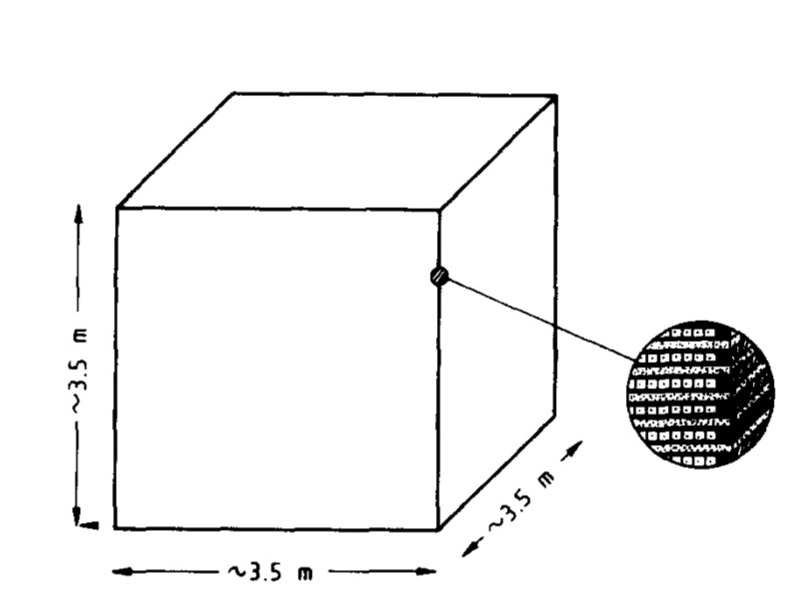
\includegraphics[width=0.49\textwidth]{figures/nusex1.jpeg}
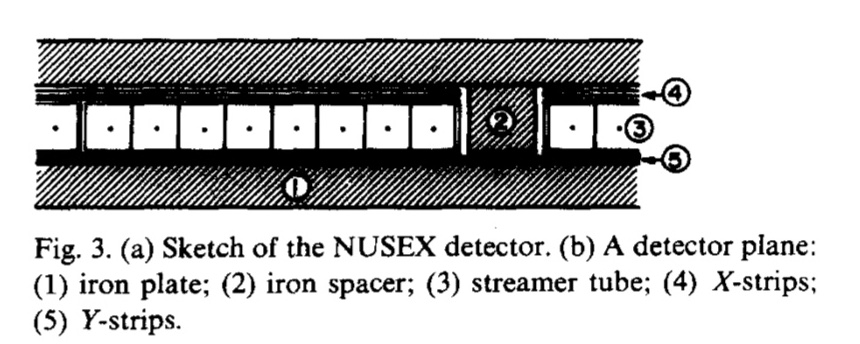
\includegraphics[width=0.49\textwidth]{figures/nusex2.jpeg}
\vspace{2mm}
\caption{A sketch of the NUSEX detector with various parts highlighted~\cite{56NUSEX}.}
\label{fig:nusex}
\end{figure}

\begin{figure}[h!]
\centering
  \centering
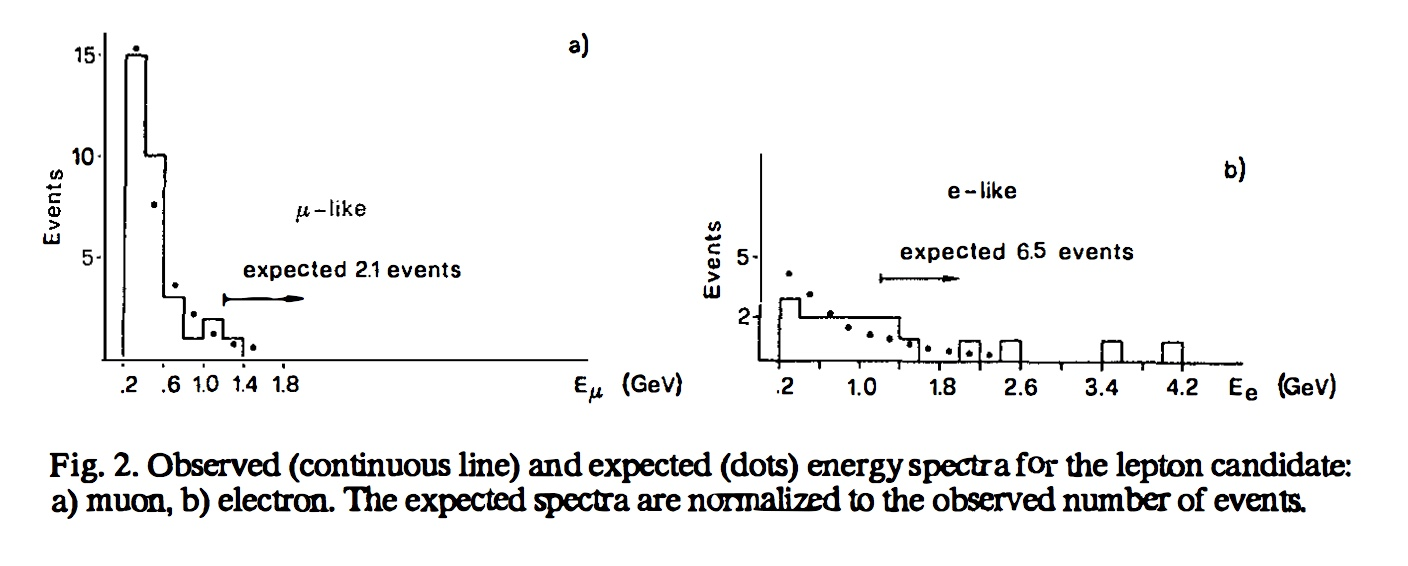
\includegraphics[width=0.5\textwidth]{figures/nusexres.jpeg}
\vspace{2mm}
\caption{Data compared to Monte Carlo for 50 neutrino events in the NUSEX and showing consistency within errors~\cite{57NUSEX}.}
\label{fig:nusexres}
\end{figure}

\subsection{KamiokaNDE}
The Kamioka Nucleon Decay Experiment (KamiokaNDE) is a 3000 ton water Cherenkov detector installed in the Kamioka mine 1000 m under the top of a mountain. The detector has the aim to study and search for nucleon decay which began operation in 1983. The Cherenkov light is detected using 1000 large PhotoMultiplier Tubes (PMTs)~\cite{58KAMIOKA}.


\if{0}
 In Japan, the Kamiokande detector (1983-1996, 3 kiloton) and Super-Kamiokande (in operation since 1996, 50 kiloton) have achieved several important scientific results, notably detection of extraterrestrial neutrinos from the Sun [40] and Supernova 1987a [41, 42], and discovery of neutrino flavor mixing and neutrino mass [6, 43]. In the K2K long baseline neutrino oscillation experiment, Super-K and a one kiloton water Cherenkov detector (1KT) provided indis- pensable data on the neutrino beam flux and its energy spectrum at the neutrino production site (using 1KT) and a location 250 km farther away (using Super-K) [22]. Super-K again is playing the role of the far detector in the ongoing T2K experiment which reported an indication of %νμ → νe oscillations in June 2011 [1].
Good paper for all of this! %https://arxiv.org/pdf/1109.3262.pdf
6, Y. Fukuda et al. (Super-Kamiokande), Phys. Rev. Lett. 81, 1562 (1998), arXiv:hep-ex/9807003.
40, K. S. Hirata et al. (KAMIOKANDE-II), Phys. Rev. Lett. 63, 16 (1989).
41, K. Hirata et al. (KAMIOKANDE-II), Phys. Rev. Lett. 58, 1490 (1987).
42, K. S. Hirata et al. (KAMIOKANDE-II), Phys. Rev. D38, 448 (1988).
43, S. Fukuda et al. (Super-Kamiokande), Phys. Lett. B539, 179 (2002), arXiv:hep-ex/0205075
Kamiokande2 was solar?
\fi
\begin{figure}[h!]
\centering
  \centering
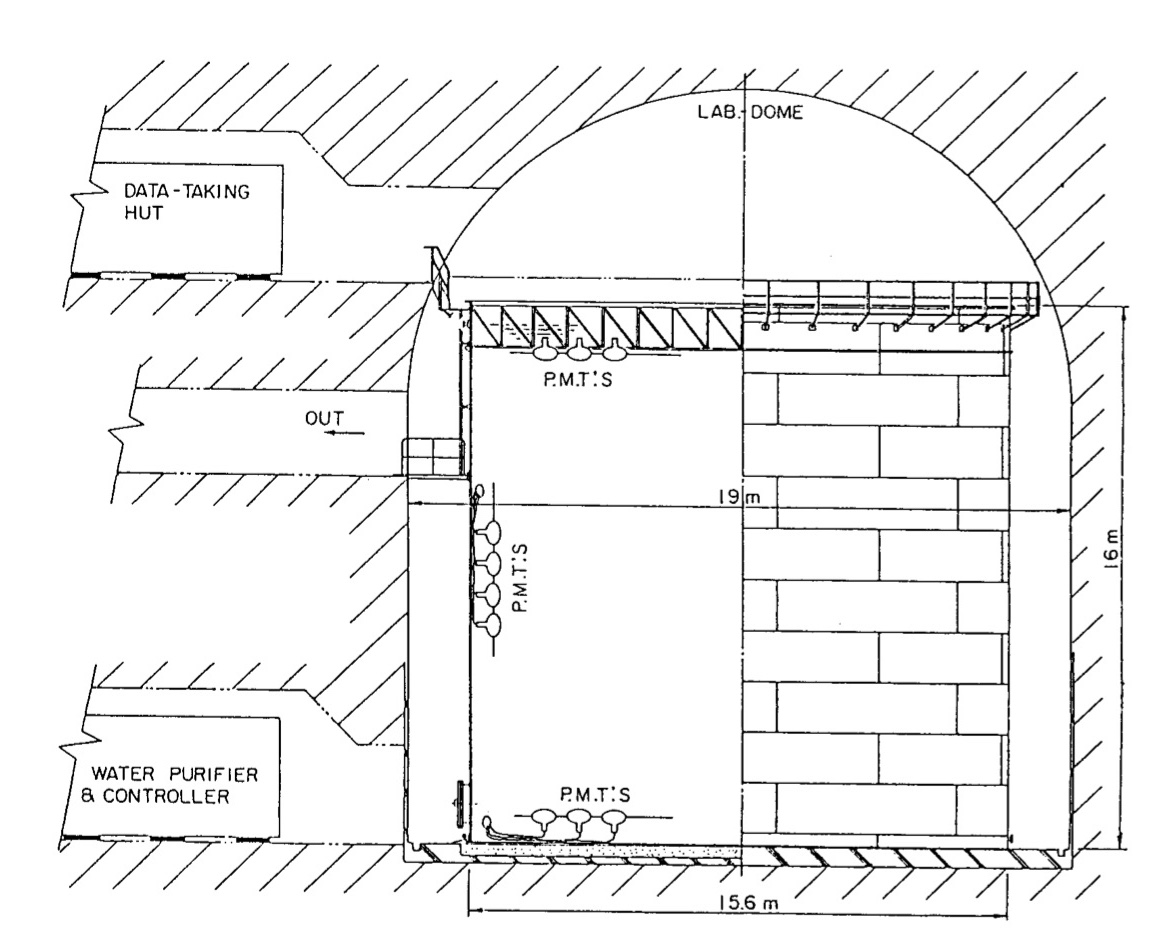
\includegraphics[width=0.5\textwidth]{figures/Kamioka1.jpeg}
\vspace{2mm}
\caption{Schematic image of the KamiokaNDE detector.~\cite{58KAMIOKA}.}
\label{fig:Kam}
\end{figure}

\begin{figure}[h!]
\centering
  \centering
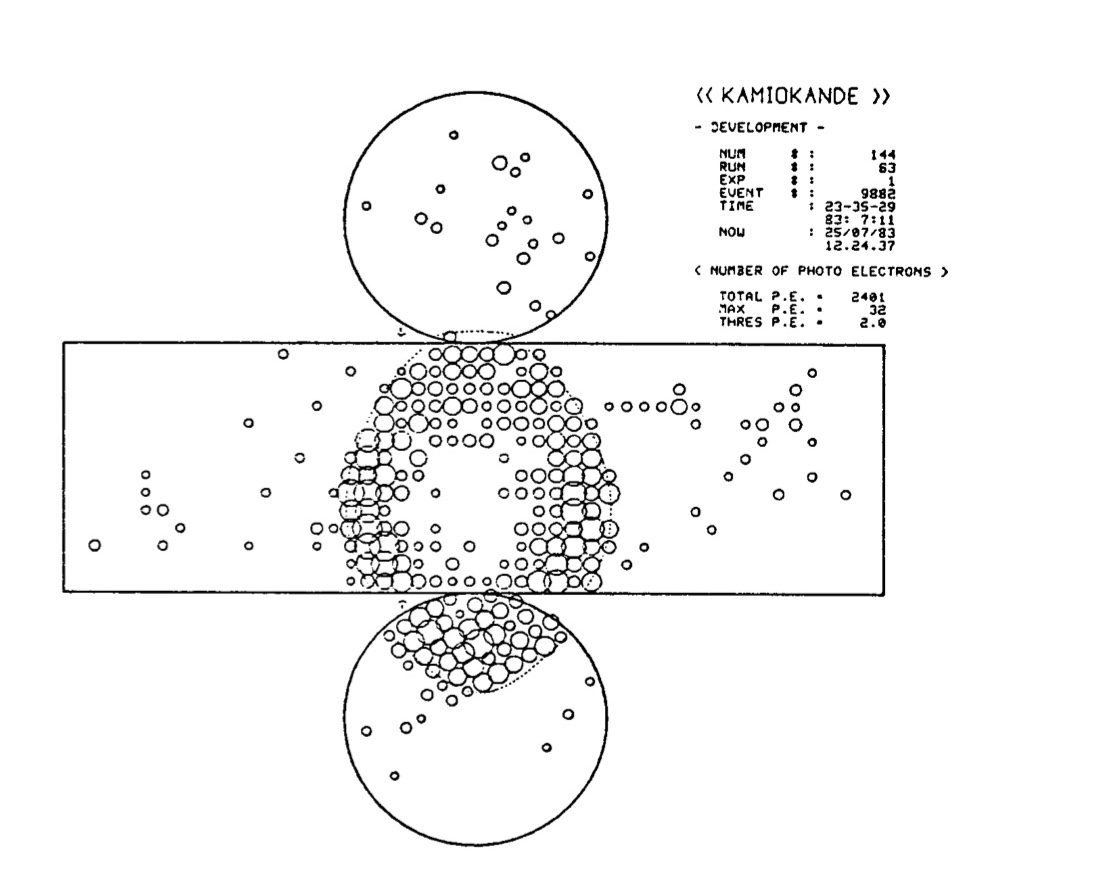
\includegraphics[width=0.49\textwidth]{figures/Kamioka2.jpeg}
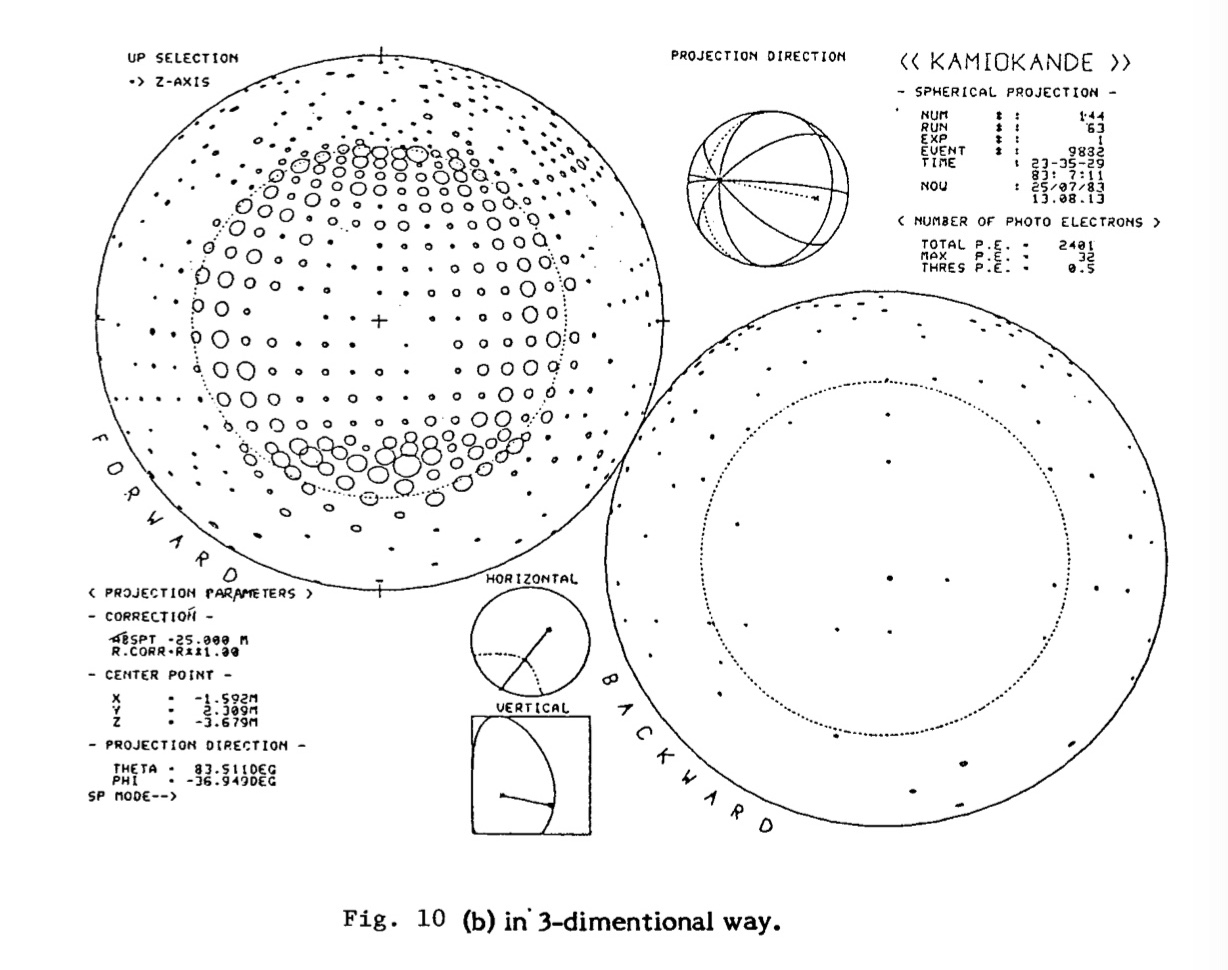
\includegraphics[width=0.49\textwidth]{figures/Kamioka3.jpeg}
\vspace{2mm}
\caption{A sample event showing Cherenkov rings produced by a muon event~\cite{58KAMIOKA}.}
\label{fig:Kam2}
\end{figure}
The main result was finding a slight discrepancy between data and simulations, seen in \FigRef{fig:Kam3}, hinting at at a possibility that atmospheric neutrinos were oscillating.
\begin{figure}[h!]
\centering
  \centering
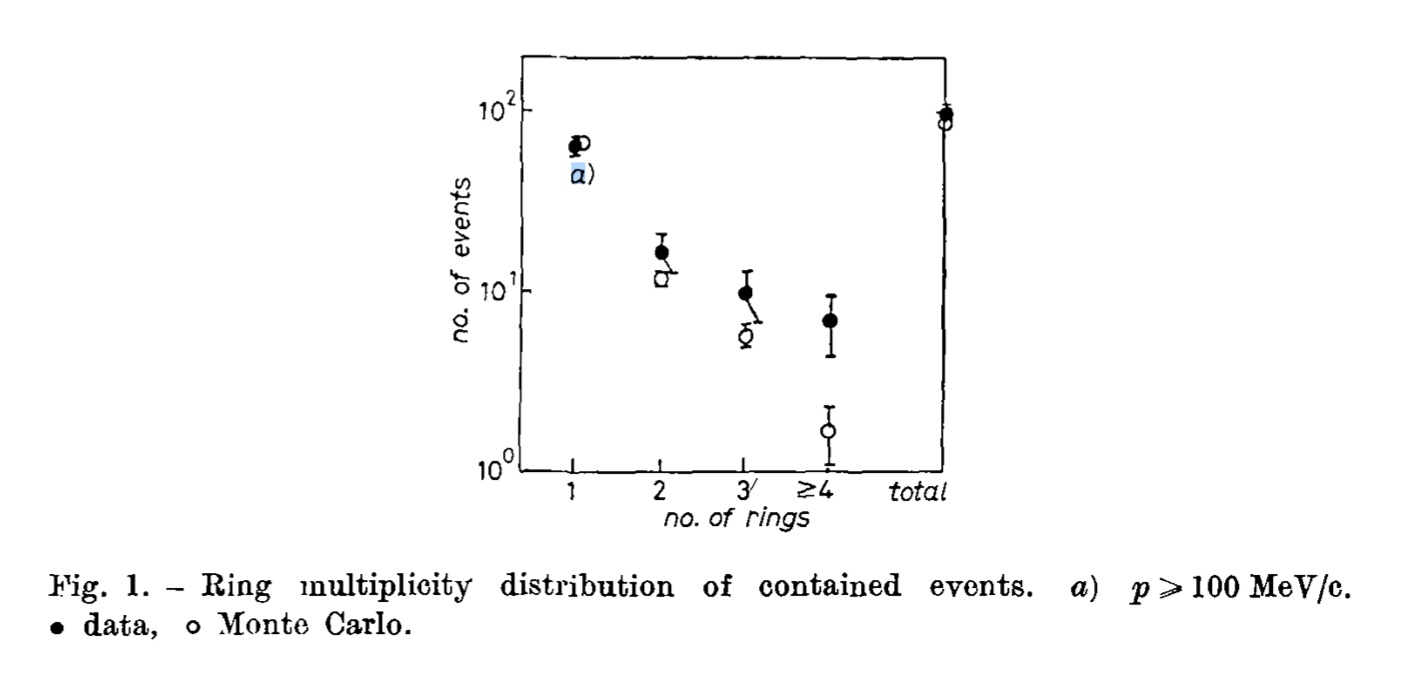
\includegraphics[width=0.49\textwidth]{figures/Kamioka4.jpeg}
\vspace{2mm}
\caption{Comparing ring multiplicity distributions between data and simulations~\cite{59KAMIOKA}.}
\label{fig:Kam3}
\end{figure}

\subsection{IMB}
The Irvine- Michigan-Brookhaven (IMB) groups build a 8 kiloton water Cherenkov detector 600 m under the Morton Salt Mine in Cleveland which began data taking in 1986. The design was similar to KamiokaNDE and managed to improve several results including improving the parameter space of neutrino oscillation~\cite{60IMB}.


\subsection{Super-Kamiokande}
Super-Kamiokande\cite{20SUPERK}, a water Cherenkov detector is located 1 km underground and consists of a cylindrical stainless steel tank holding 50 ktons of ultra-pure water, performed the first experimental observation that the neutrino has non-zero mass\cite{10Fukuda} and also managed to detect strong evidence of muon neutrino oscillation to tau neutrinos from the analysis of atmospheric neutrinos interacting in the water target~\FigRef{fig:SK2}. The deviation from 1 shows the discovery of neutrino oscillations and the lines show the expected shape for oscillation from muon neutrinos to tau neutrinos~\cite{10Fukuda}. It also shows that electron-like events have no significant variation in length over neutrino energy where at large length over neutrino energy muon-like events have come to close to half of the initial rate.

\begin{figure}[h!]
\centering
  \centering
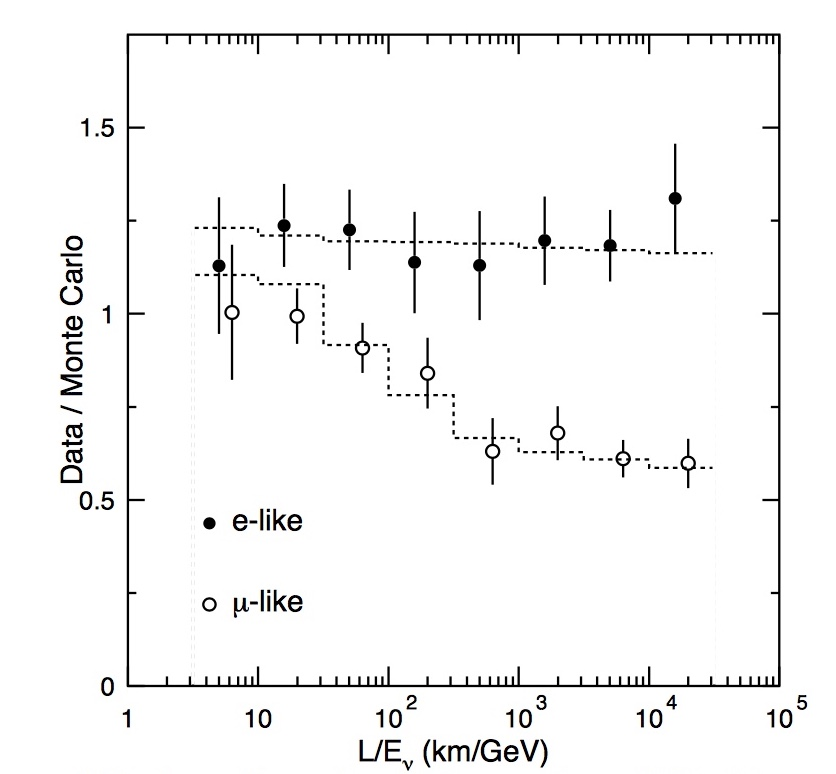
\includegraphics[width=0.49\textwidth]{figures/simuSK2.jpeg}
\vspace{2mm}
\caption{Comparison of the ration of data vs Monte Carlo vs length over neutrino energy for fully contained atmospheric electron-like and muon-like events~\cite{10Fukuda}.}
\label{fig:SK2}
\end{figure}

\begin{figure}[h!]
\centering
\begin{subfigure}{.5\textwidth}
  \centering
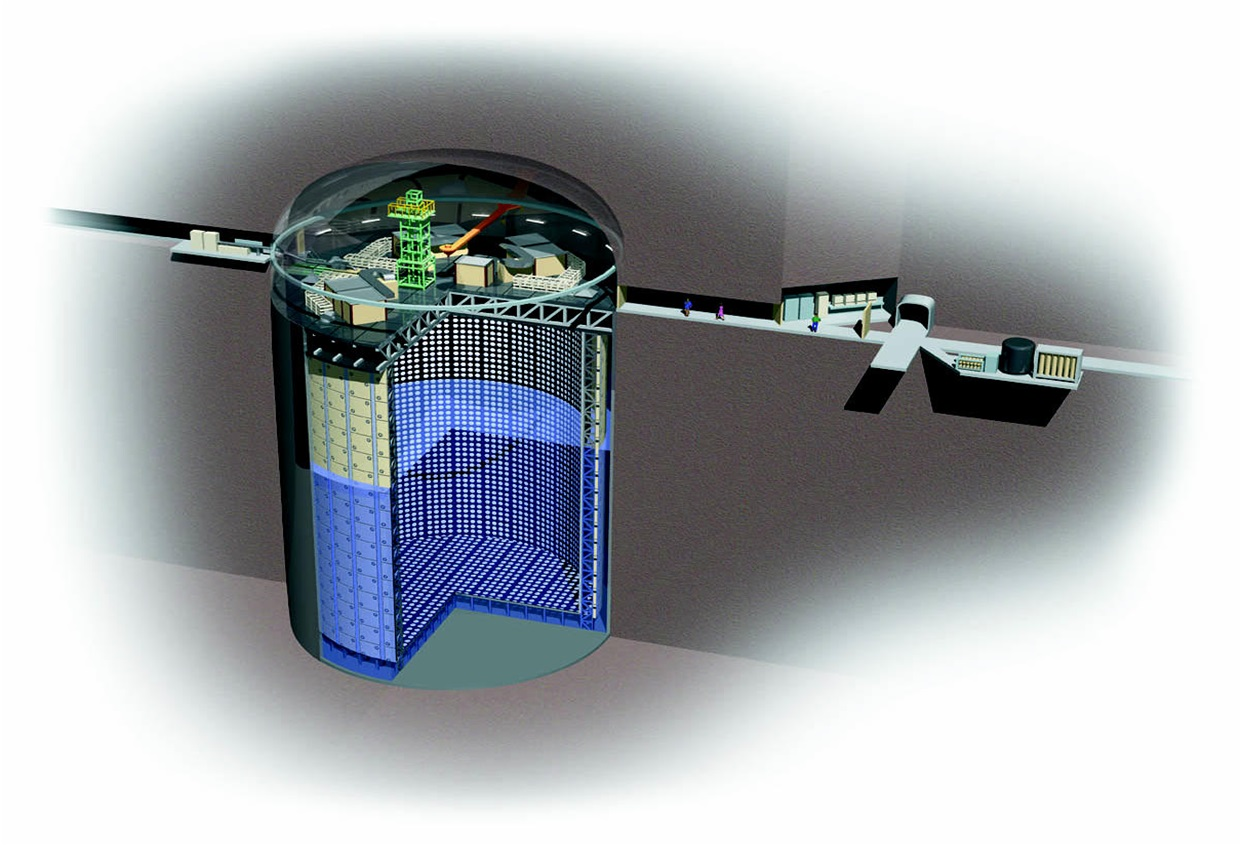
\includegraphics[width=\textwidth]{figures/SK3D.jpg}
\vspace{2mm}
  %\label{fig:sub1}
\end{subfigure}%
\begin{subfigure}{.5\textwidth}
  \centering
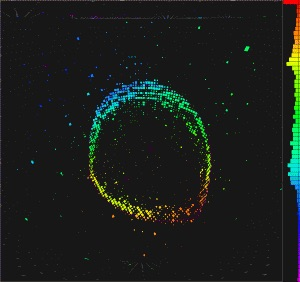
\includegraphics[width=0.7\textwidth]{figures/SuperKMuon-300x282.jpg}
\vspace{2mm}
  %\label{fig:sub2}
\end{subfigure}
\vspace{2mm}
\caption{Left) A schematic of the Super-K detector., Right) Event recorded in Super-K.}
\label{fig:SK}
\end{figure}
% http://t2k-experiment.org

\subsection{MACRO}
The Monopole, Astrophysics and Cosmic Ray Observatory (MACRO) was combined of liquid scintillation counters, limited streamer tubes and nuclear track detectors allowing it to searching for signs of magnetic monopoles, as well as being able to operate as a neutrino detector as well as search for other phenomena. Data was taken between 1995 until 2000 and by measuring neutrin induced muons, the MACRO managed to aid in the discovery of atmospheric neutrino oscillation~\cite{62MACRO}

\begin{figure}[h!]
\centering
  \centering
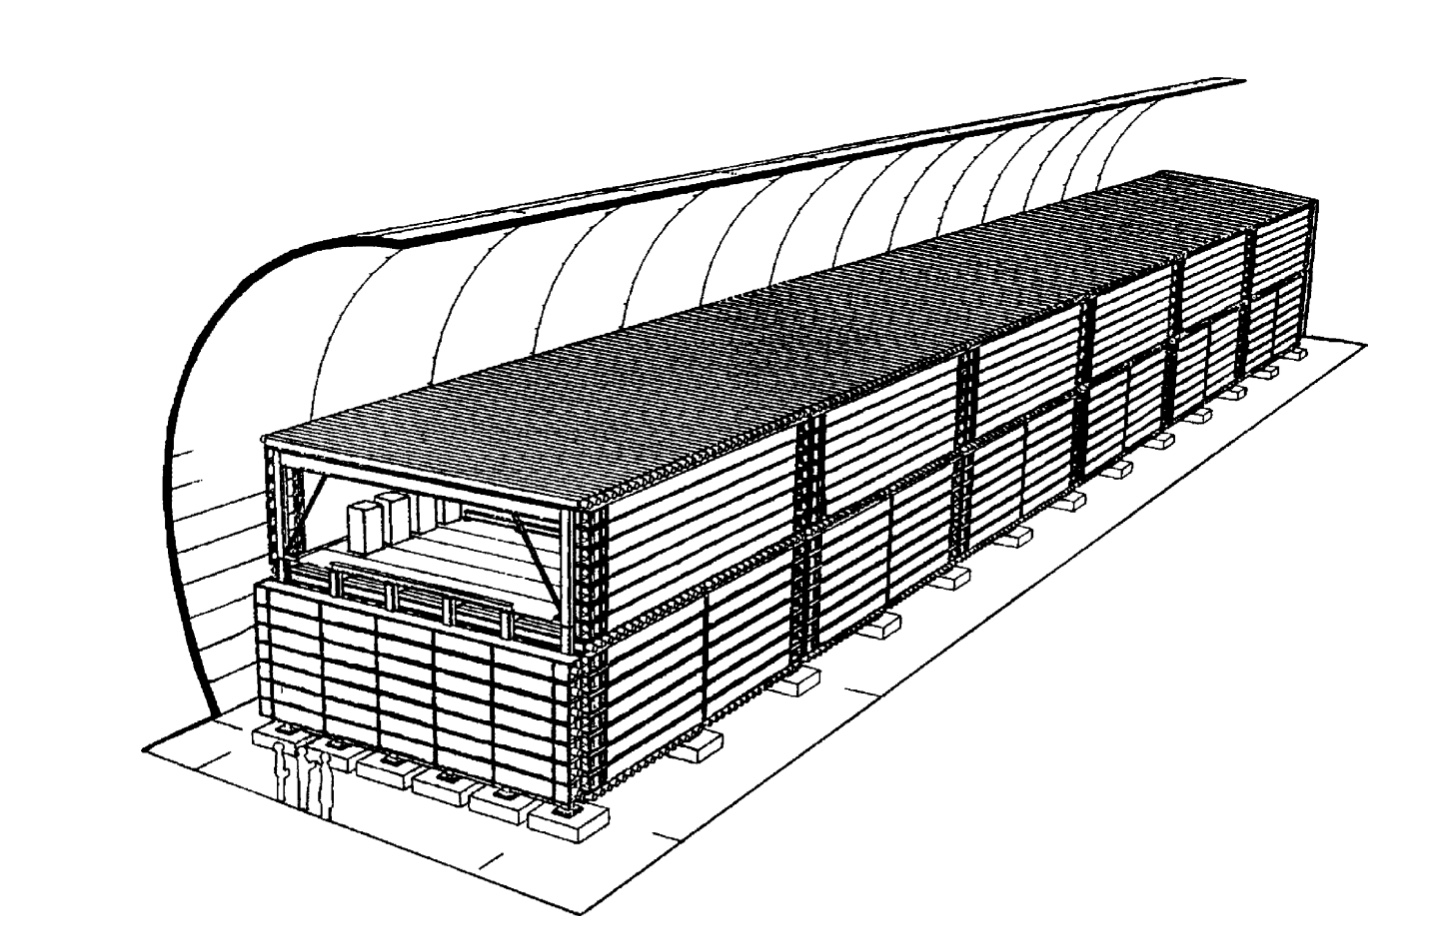
\includegraphics[width=0.49\textwidth]{figures/MACRO.jpeg}
\vspace{2mm}
\caption{Schematic of the MACRO~\cite{61MACRO}.}
\label{fig:Kam3}
\end{figure}

\section{Solar}
The mechanism for neutrino generation in the sun was briefly discussed in subsection~\ref{subsection:Missing}.
Solar neutrinos are interested for both allowing a unique way of probing the internal solar reactions as well as providing a very baseline combined with energies of around $1 MeV/c$ allowing probing of mass differences in the range of $\Delta m^2 \approx 1-^{-10} eV^2$ through neutrino oscillation, see equation~\ref{eq:twoPNeutrinoosc}. Based on current experimental values these experiments are sensitive for $\theta_{12}$ and $\Delta m_{12}^2 $

Mention best values and different hierarchy?

\subsection{Super-Kamiokande}

Super-Kamiokande, as described above, could thanks to its design also be used for solar neutrino studies and extended the neutrino oscillation analysis to lower mass difference values as well as performed solar interaction measurements~\cite{64SuperK}.

\subsection{SNO}
The Sudbury Neutrino Observatory (SNO)~\cite{Fix6} was build to make a definite measurement of solar neutrinos following the measurements taken by the Homestake experiment~\cite{9Davis}. It utilized PMT (Photo Multiplier Tubes) to measure Cherenkov radiation produced by neutrino interactions in the detectors 1000 ton ultra-pure heavy water volume. The whole detector is placed 2 km underground to minimize background interactions. It expanded on looking for a specific energy range for cosmic rays, Boron decay, to becoming a generic neutrino detector meaning that other atmospheric and cosmic neutrinos became background events for measuring solar neutrinos. The experiment has a unique ability to separate the reactions between electron neutrino charge current (CC), neutral current interactions (NC) with all flavours of neutrinos and with electron scattering (ES). With this observed neutrino flux observed through CC reactions could be compared to that of the ES  and NC to provide evidence for a neutrino flavour change regardless of the predictions of solar modes.

The experiment clearly showed a significant difference in flux between CC interactions, only available with electron neutrinos compared to expected and compared to the NC and ES interactions. The result can be seen in \FigRef{SNO2}.

\begin{figure}[h!]
\centering
\begin{subfigure}{.5\textwidth}
  \centering
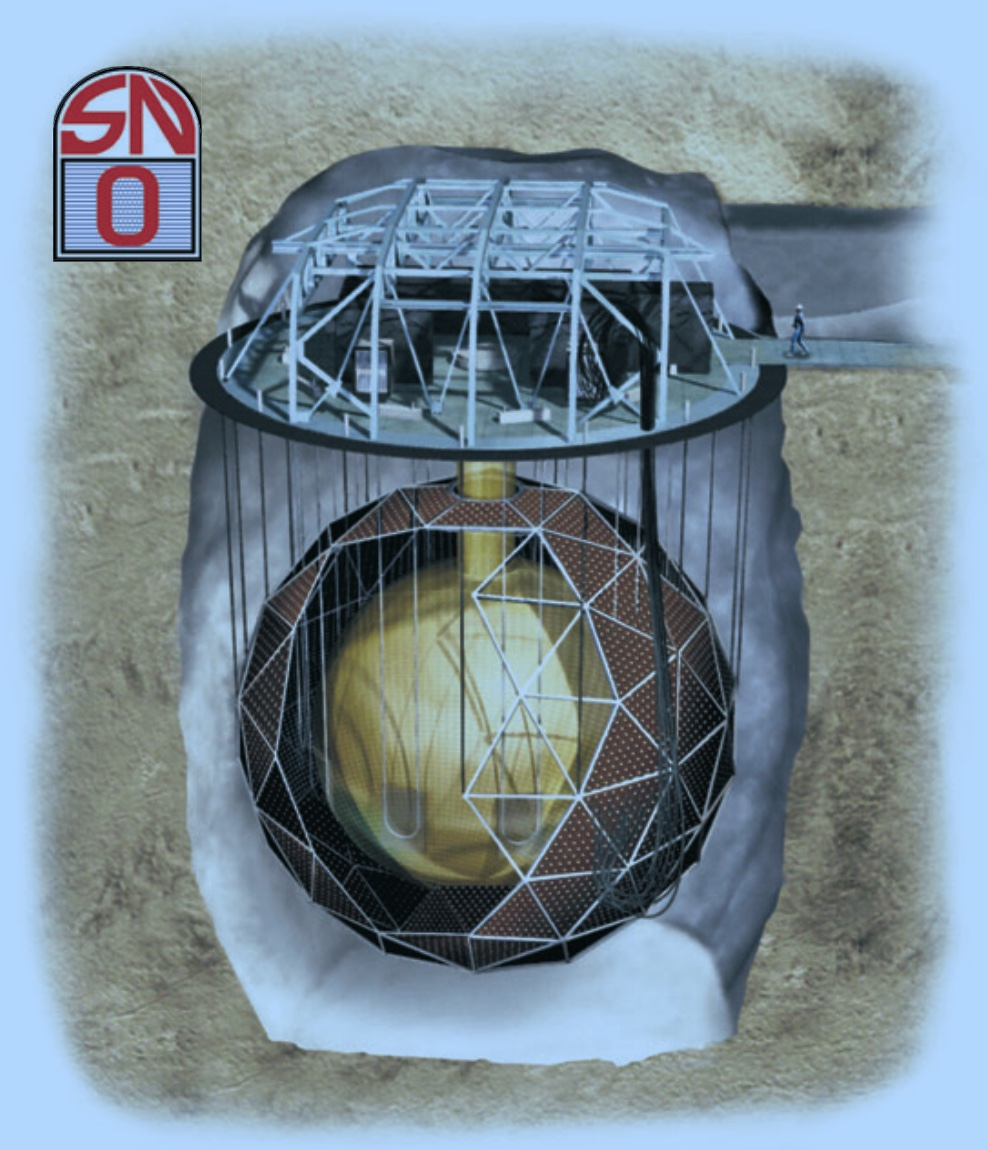
\includegraphics[width=0.7\textwidth]{figures/sno.jpeg}
\vspace{2mm}
  %\label{fig:sub1}
\end{subfigure}%
\begin{subfigure}{.5\textwidth}
  \centering
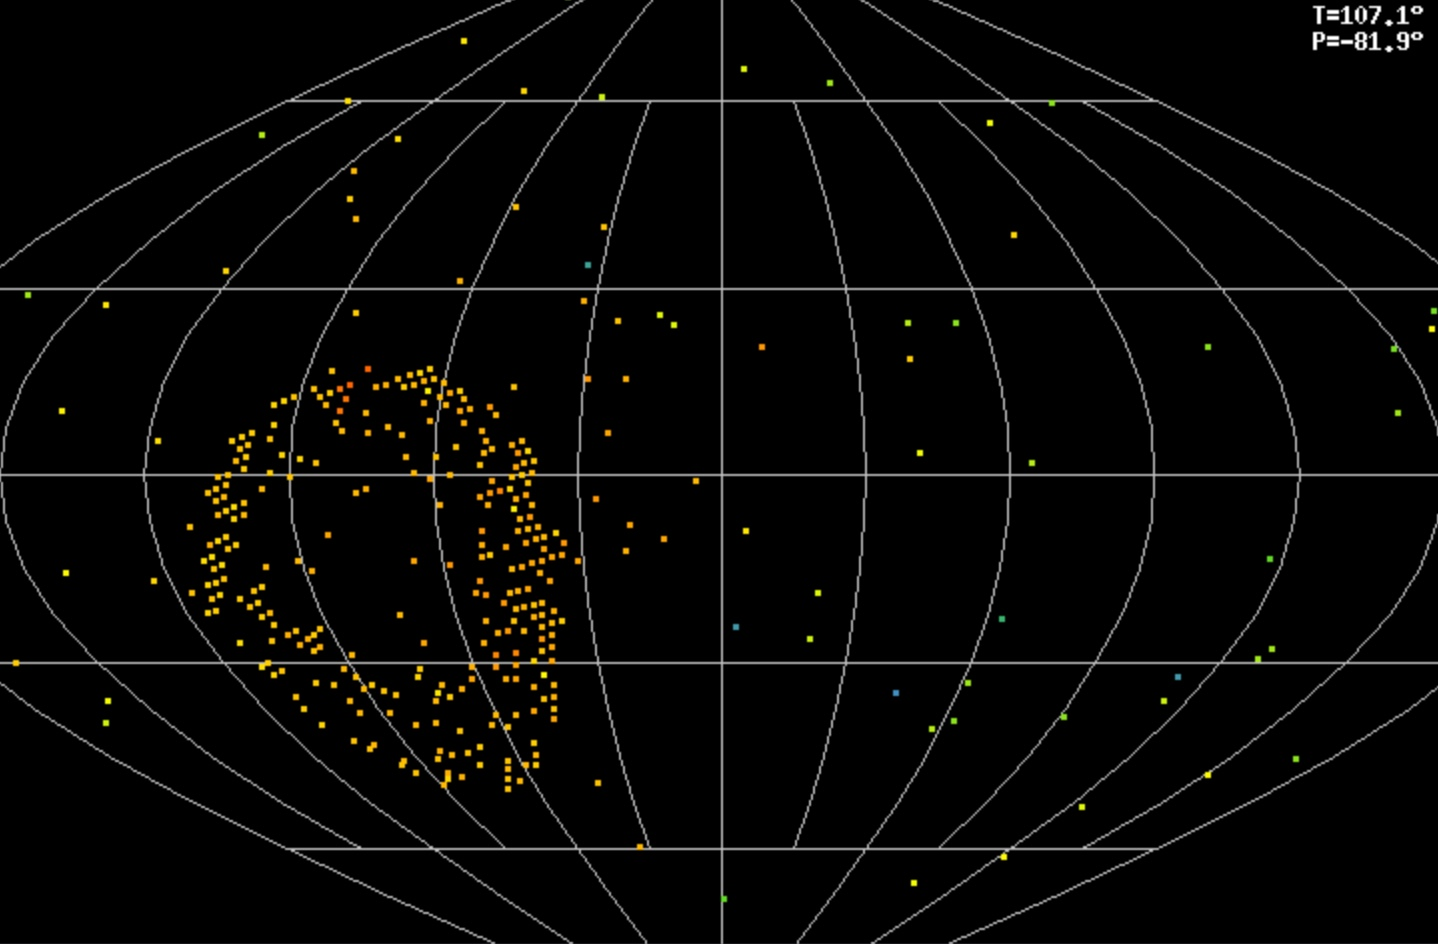
\includegraphics[width=\textwidth]{figures/SNOmuonEvent.jpeg}
\vspace{2mm}
  %\label{fig:sub2}
\end{subfigure}
\vspace{2mm}
\caption{Left) A schematic drawing of the SNO detector~\cite{Fix6}, Right) Cherenkov light recorded from a muon created by interaction of an atmospheric neutrino in the heavy water.}
\label{fig:SNO}
\end{figure}

\begin{figure}[h!]
\centering
  \centering
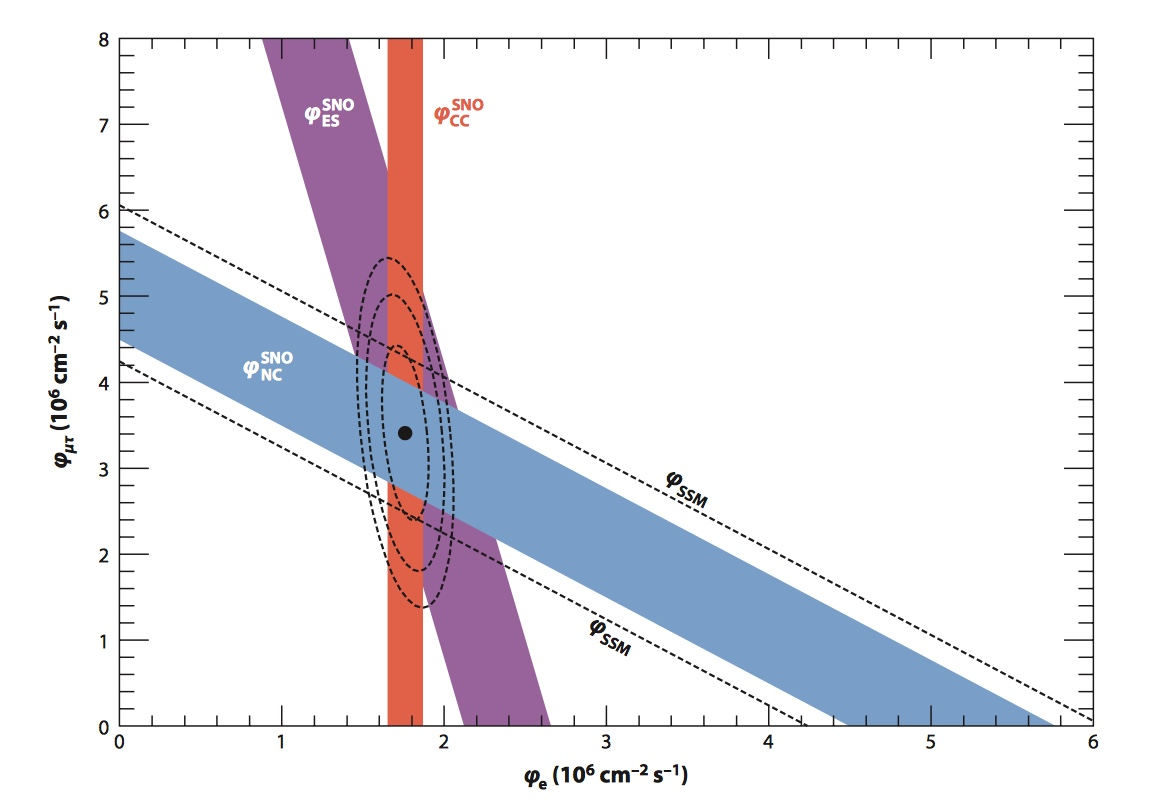
\includegraphics[width=0.49\textwidth]{figures/snoSpec.jpeg}
\vspace{2mm}
\caption{The flux of solar neutrinos of $\mu$ or $\tau$ flavour vs flux of electron neutrinos measured in SNO from the three reactions, CC in red, ES in purple and NC in blue.The diagonal dashed lines show the prediction from the Standard Solar Model. The coloured bands intersect at the fit values for all fluxes indicating that they are consisted with neutrino flavour transformation with no distortion in the solar neutrino energy spectrum. ~\cite{Fix6}.}
\label{fig:SNO2}
\end{figure}

The experiment is currently replacing the heavy water with liquid scintilator and renaming itself as SNO+~\cite{42SNO+}.

\subsection{Borexino}
Started data taking in May 2007. Ongoing. measure solar neutrinos very precise measurements of neutrino fluxes from sun.limits on charge non conservation. limits on sterile neutrinos and geoneutrinos. pep solar neutrinos first measurement.

Borexino is a liquid scintillator detector making it more sensitive, especially to the low energetic solar neutrinos, than Cherenkov techniques but lacks the ability to detect directionality of incoming particles requiring an extremely low radioactive contamination of the scintillator media. This is handled by containing the detector within shielding material and utilizing ultra pure materials~\cite{63Borexino}. The scintillating light is then read out by PMTs uniformly distributed around the active volume seen in \FigRef{fig:borexino}.

\begin{figure}[h!]
\centering
  \centering
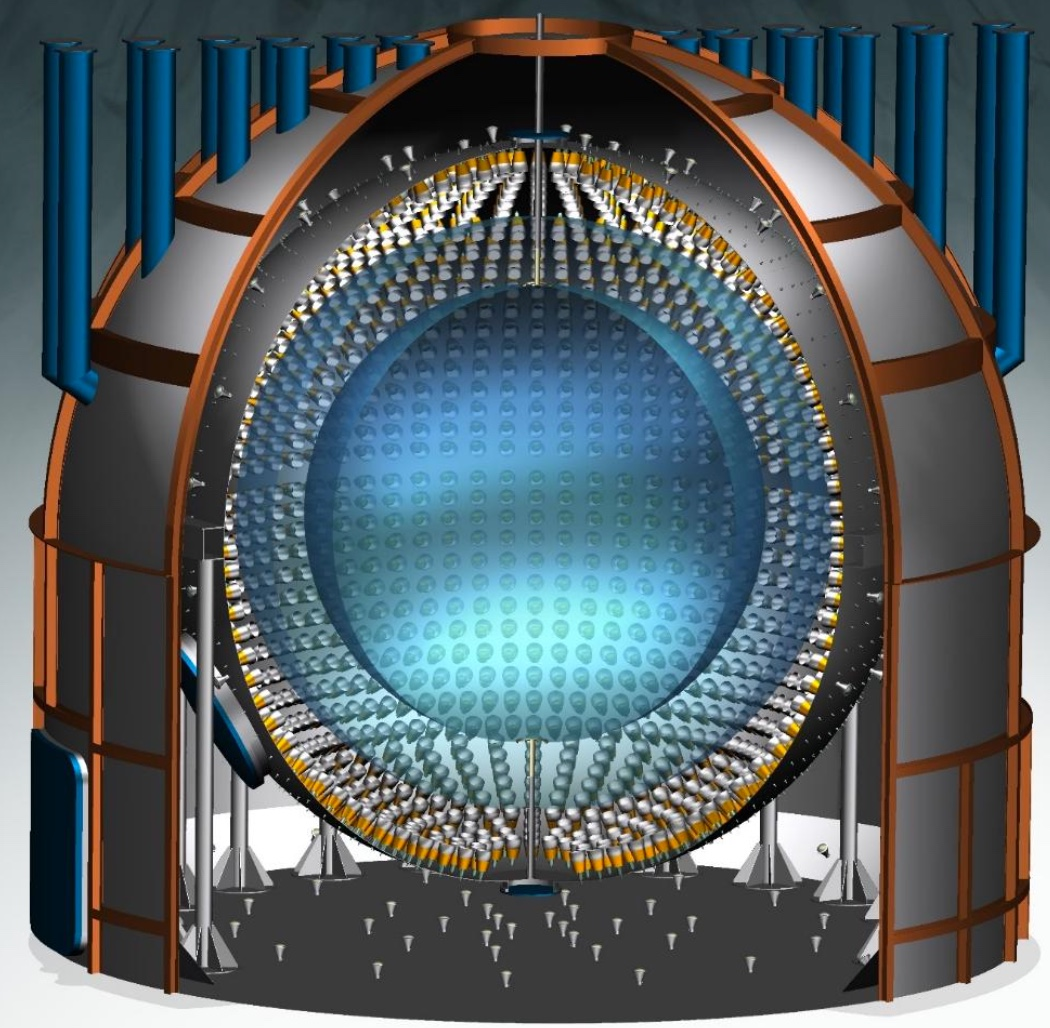
\includegraphics[width=0.49\textwidth]{figures/borexino.jpeg}
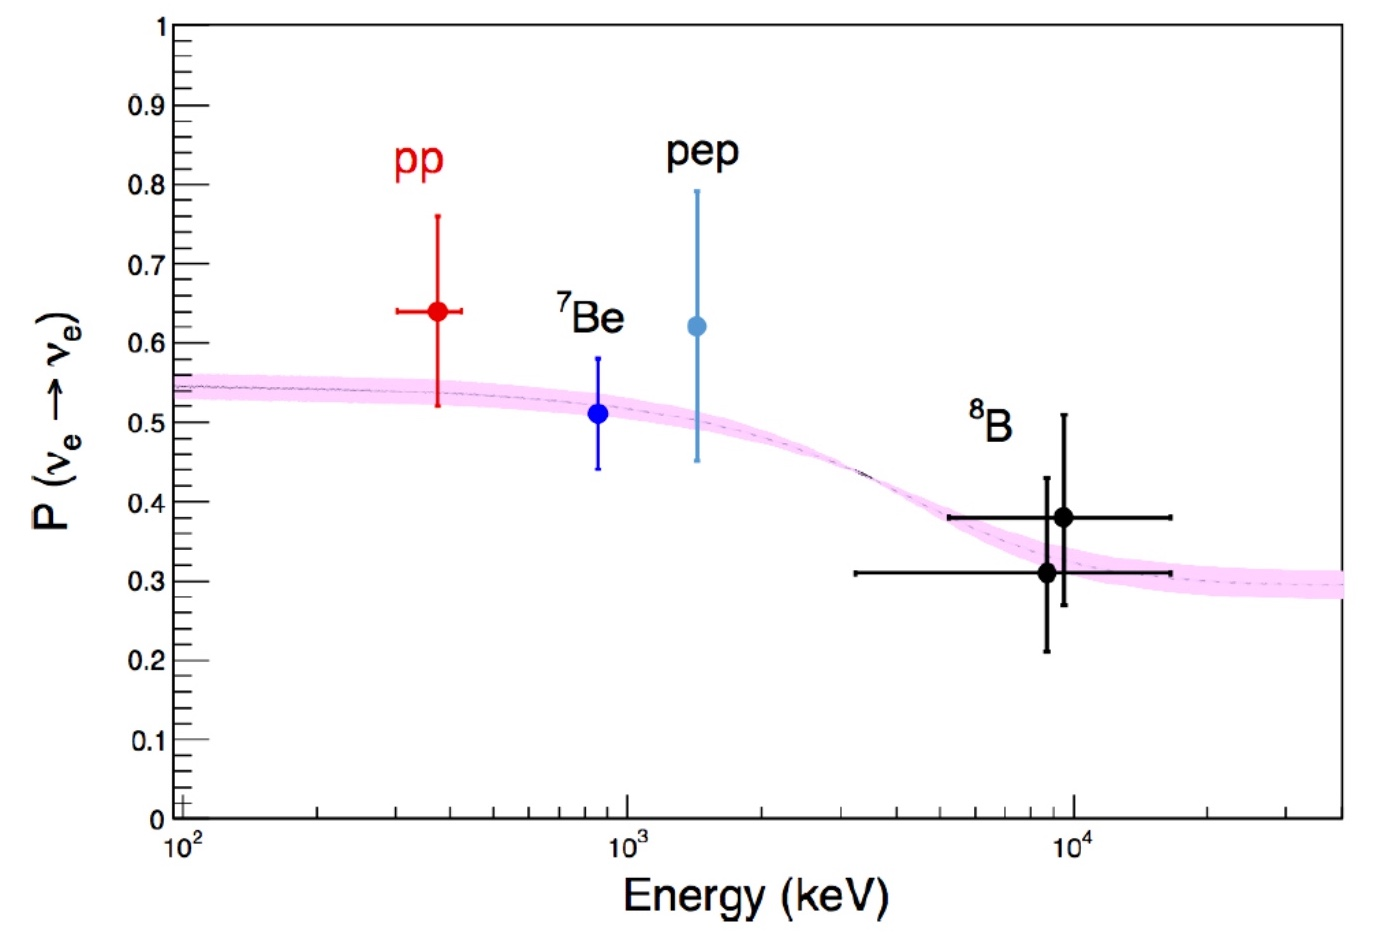
\includegraphics[width=0.49\textwidth]{figures/borexino3.jpeg}
\vspace{2mm}
\caption{(Left) Schematic of the Borexino experiment~\cite{63Borexino}. (Right) Electron neutrino survival probability as a function of neutrino energy according representing different neutrino solar production channels both from the Solar standard model and measurements from the Borexino experiment~\cite{63Borexino}.}
\label{fig:borexino}
\end{figure}

quote!

5. Conclusion
\textbf{The most recent solar and terrestrial neutrino results stemmed from Borexino have further reinforced the ultra-low background achievements of this experiment, an exceptional breakthrough in the field of techniques for rare processes search. The 7Be, 8B, pep and the very recently measured pp components have all been detected (together with a tight upper limit on CNO), leading to the validation of the MSW-LMA oscillation paradigm in the entire energy regime of the solar neutrinos, strengthened also by the determination of the absence of day-night asymmetry in the 7Be flux. Very remarkably, Borexino performed this validation with its own data, without the need to resort to the results of other solar neutrino experiments.
Finally, the highly significant measurement of the terrestrial neutrinos not only complements the physics potentiality of the detector, but points towards a future new direction of research in the studies of the interior of the Earth.}

\section{Accelerator}
Currently accelerator facilities can produce muon and electron neutrinos and anti neutrinos from accelerated protons. Protons are accelerated in a particle accelerator where the energy of the protons is related to the energy of the neutrinos. The proton beam is then directed at a target where the protons interact with the target material, producing a large number of secondary pions (among other particles). Shaped magnetic fields, so called focusing horns, are used to select out pions of the preferred charge (positive for a neutrino beam, negative for an antineutrino beam) in a specific momentum range and focus them into a collimated beam. The beam is directed into a long decay volume, where the pions decay into muons and (anti)neutrinos. At the end of the decay volume there is a large mass of material which absorbs all the particles except the neutrinos. This provides a nearly pure beam of muon-neutrinos (or muon-antineutrinos if negatively charged pions are selected). There is some inevitable contamination from antineutrinos in the neutrino beam or neutrinos in the antineutrinos beam and from electron-neutrinos, mostly because the original pion beam also includes some kaons, which can decay to produce electron-neutrinos as well as from muon interactions. To differentiate between these accelerator-based neutrino experiments, like reactor experiments, generally use a near detector as well as a far detector. This configuration allows comparison of the neutrino beam at the near detector with the far detector to determine if there has been any neutrino oscillation.

The advantage of accelerator neutrinos are that the energy range is well known and can be quite well tailored, the flux is huge compared to other methods. However the energy distribution will be quite wide because of the decay processes involved. It is also hard to produce a clean beam without background, muon neutrinos without electron neutrinos. However, for oscillation experiments this can be a good thing, see subsection \ref{subsec:nuFACT}. Based on current experimental values these experiments are sensitive for $\theta_{23}$ and $\Delta m_{23}^2 $

\subsection{Historical experiments}
%The European Organization for Nuclear Research, (CERN) has had accelerator neutrino experiments and some based around magnetised volumes to provide change identification of particles. 

The European Organization for Nuclear Research (CERN) Dortmund Heilelberg Saclay Warsaw (CDHSW)~\cite{40CDHSW} experiment was designed to study neutrino interactions in iron using the CERN SPS neutrino beam line. The experiment consisted of two similar detectors at different distances from the interaction vertex 130 m and 885 m~\cite{40CDHSW}.The detectors were built designed to combine the functions of a muon spectrometer and a hadron calorimeter. It consisted of 19 toroidal magnetised iron modules, with an average field of 1.65 T, separated from each other by wire drift chambers and had a mass of 1250 tons. In the end of the experiment a liquid hydrogen tank was placed in front of the experiment to study neutrino interactions in hydrogen. This is one of the first MINDs (Magnetised Iron Neutrino Detectors).

The CHARM Collaboration (CERN-Hamburg-Amsterdam-Rome-Moscow Collaboration) proposed to study neutrino-nucleon neutral current interaction as well as muon polarisation. It took data from 1978 to 1991 and  was comprised of a fine-grained target calorimeter made up of 78 subunits each surrounded by a frame of magnetized iron for muon identification and spectrometry~\cite{68CHARM}.

The CCFR (University of Chicago, Columbia University, Fermilab, and the University of Rochester) detector installed at Fermilab consists of an 18 m long 690 ton neutrino target calorimeter and followed by an iron toroid spectrometer. The calorimeter consists of 168 iron plates, each 3m x 3m x 5.1cm, with liquid scintillation counters spaced between every two plates and drift chambers spaced every four plates. It provided among other things, precision measurements fro neutrino-nucleon scattering~\cite{67CCFR}. The experiment was continued through the NuTeV experiment which expanded results using the same detector. CCFR took data from 1979 to 1988, NuTeV started in 1996 and continued until 2003.

\subsection{NOMAD}
The Neutrino Oscillation Magnetic Detector (NOMAD)~\cite{NOMADexp}, also using the CERN SPS neutrino beam line, searched for $\nu_\mu \rightarrow \nu_\tau$ oscillation by detecting $\tau$ appearance. Its goals were to measure the momenta of charged particles and identify and measure electron, photons and muons. By the detector design it was also possible to look for $\nu_\mu \rightarrow \nu_e$ oscillation. Compared to the modular design of CDHS, NOMAD had drift chambers and other subdetectors contained inside a dipole magnet at 0.4 T.

%\textbf{RESULTS?}
\begin{figure}[h!]
\centering
  \centering
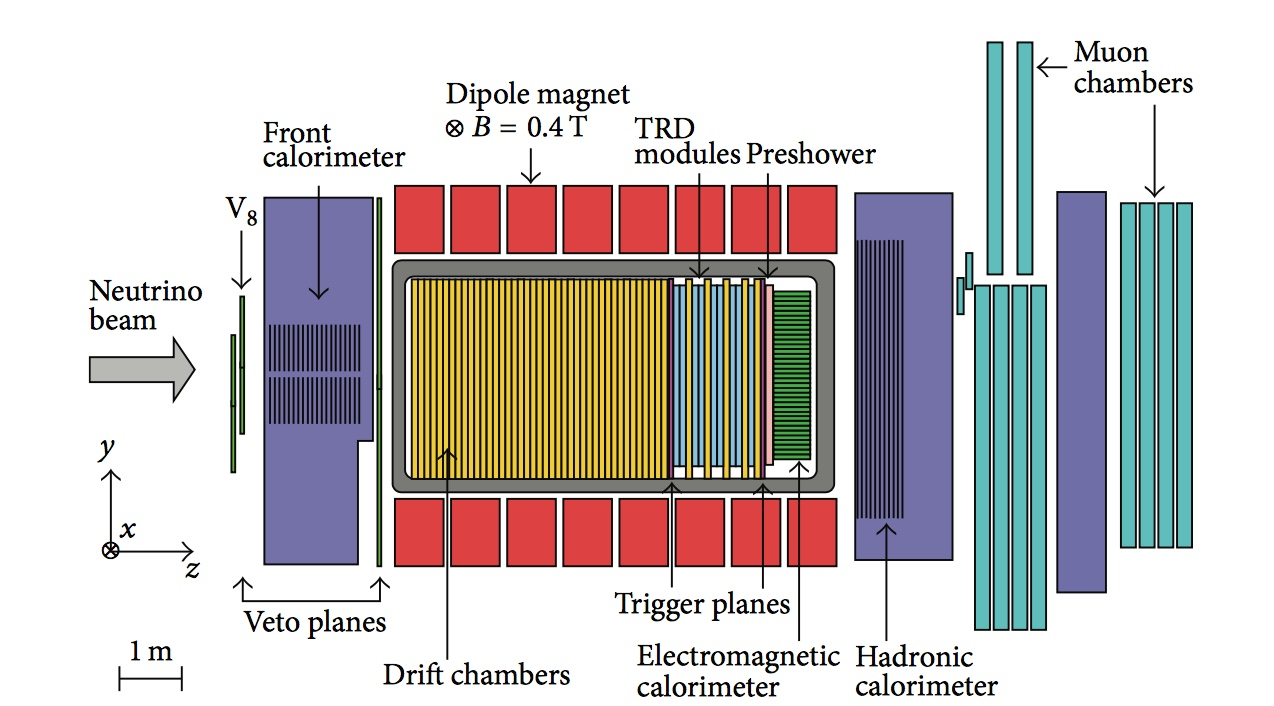
\includegraphics[width=0.7\textwidth]{figures/NOMAD2.jpeg}
\vspace{2mm}
\caption{A sideview of the NOMAD detector~\cite{69NOMAD}.}
\label{fig:NOMAD}
\end{figure}

\subsection{K2K}
After the success of Super-Kamiokande, the KEK to Kamiokande (K2K) experiment\cite{22K2K} was created with the main difference of using a well understood muon neutrino beam pointing at the Super-Kamiokande detector at a distance of 250 km. It was the first neutrino oscillation measurement where both the source and detector were controlled, it observed the disappearance of muon neutrinos into tau neutrinos and found results that were consistent with Super-Kamiokande.

K2K, the set up seen in~\FigRef{fig:K2K} and ran from 1999 to 2004, used a neutrino beam with a wide spectrum peaked at 1 GeV based on a 12 GeV proton synchrotron beam which interacts with an aluminium target and focused through two horns and allowed to decay in a 200 m long decay pipe. This creates a 98\% pure muon neutrino beam with around 1\% contamination of anti muon neutrinos and around 1\% electron and anti-electron neutrinos. Understanding the beam is required for looking at $\nu_\mu \rightarrow \nu_e$ appearance requires a good understanding of the beam composition. To do this a 1-kiloton water Cherenkov near detector,  a scaled-down version of Super-Kamiokande, is used to measure the neutrino spectrum which is then extrapolated using Monte Carlos simulated data to provide a neutrino spectrum at Super-Kamiokande detector.

\begin{figure}[h!]
\centering
  \centering
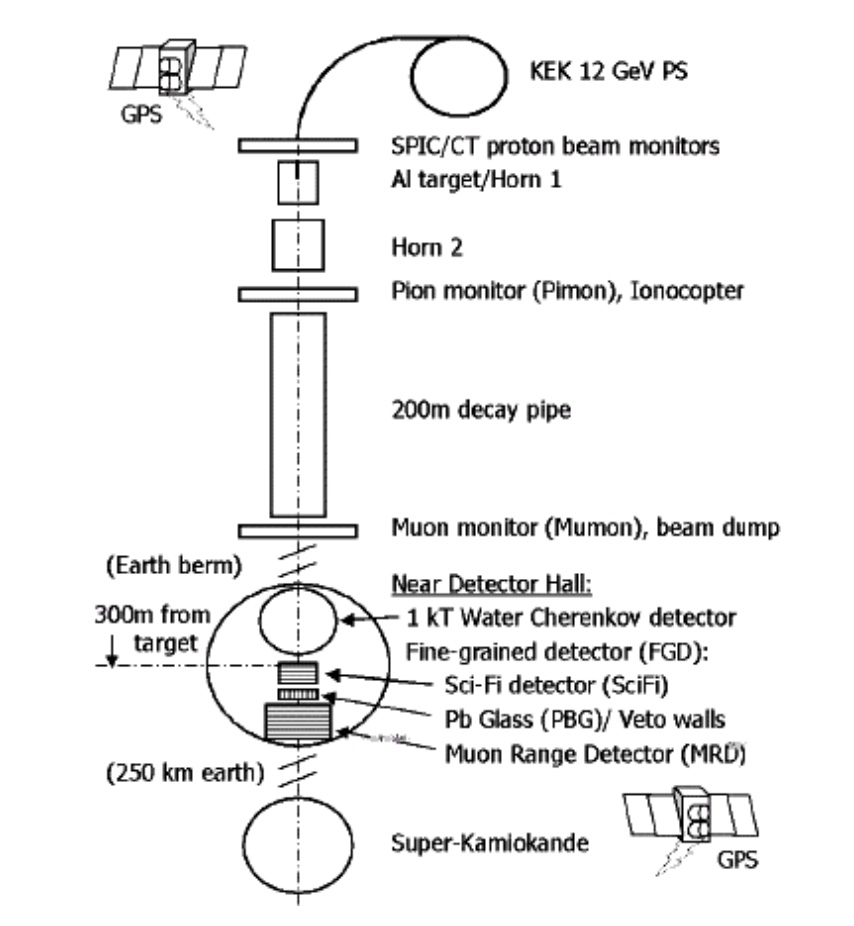
\includegraphics[width=0.5\textwidth]{figures/KEK.jpeg}
\vspace{2mm}
\caption{A schematic view of the K2K experiment Super-K~\cite{70K2K}.}
\label{fig:K2K}
\end{figure}

\subsection{MINOS}
%\url{http://www-numi.fnal.gov/Minos/minospub.txt}

The Main Injector Neutrino Oscillation Search (MINOS)~\cite{MINOS} is a muon neutrino disappearance experiment, consisting of one near (1km from the target) and one far detector (735km from the target) and using the NuMI~\cite{19NuMI} beam at Fermilab. 

The two detectors have been designed to be as similar as possible to minimize any systematic errors in comparing the observed neutrino spectra in the two detectors. They are both constructed of planes with two magnetised steal plates with a layers of scintillator in-between to measure charged particles and allow discrimination and of charge and measurement of the momentum. The far detector is composed of 486 octagonal plates with a diameter of 8 meters and total length of 30 meters providing a total mass of 5400 tons. The near detector contains only 282 planes, slightly squashed octagonal planes at 3.8 meters $\times$ 4.8 meters. MINOS showed results consistent with Super-Kamiokande and the K2K experiments. 

After MINOS the next step using the NuMI~\cite{19NuMI} beam is the NOvA~\cite{18nova} experiment, which is also an electron neutrino appearance experiment and hopes to be able to determine the mass hierarchy of neutrinos.

The MINERvA (Main INjector ExpeRiment $\nu$-A)experiment \cite{39minerva} will also use the NuMI~\cite{19NuMI} beam to study neutrino-nucleus scattering to improve models of neutrino-nucleus scattering to reduce systematic uncertainties in results from oscillation experiments.

MiniBooNE\cite{41MiniBooNE} continued on what was started by MINOS but had the principle aim on improving neutrino mass measurements.

\subsection{T2K}
\textbf{Correct after Pauls comments and add data.}

\textbf{Here or in chap 3?}

After the success of KEK, a similar baseline was constructed with the T2K-experiment\cite{21T2K},  a long-baseline neutrino oscillation experiment with a more powerful beam from the JPARC facility at Tokai to Super-Kamiokande, at a distance of 295 km with a near detector at hall 280 meters, in Tokai, from the target, see figure\ref{fig:T2K}

The neutrino beam comes from an initial 30 GeV/c proton beam which is passed through a horn fired onto a graphite target. After the target the secondary beam is passed through two magnetic horns and focused into a decay volume before passing the beam stopper. From here there is $\approx180$ meters of soil until hitting the near detector hall. This means that the near detector is comprised of only neutrinos with an expected flux as seen in \FigRef{fig:ND280Flux}. 

\begin{figure}[h!]
\centering
  \centering
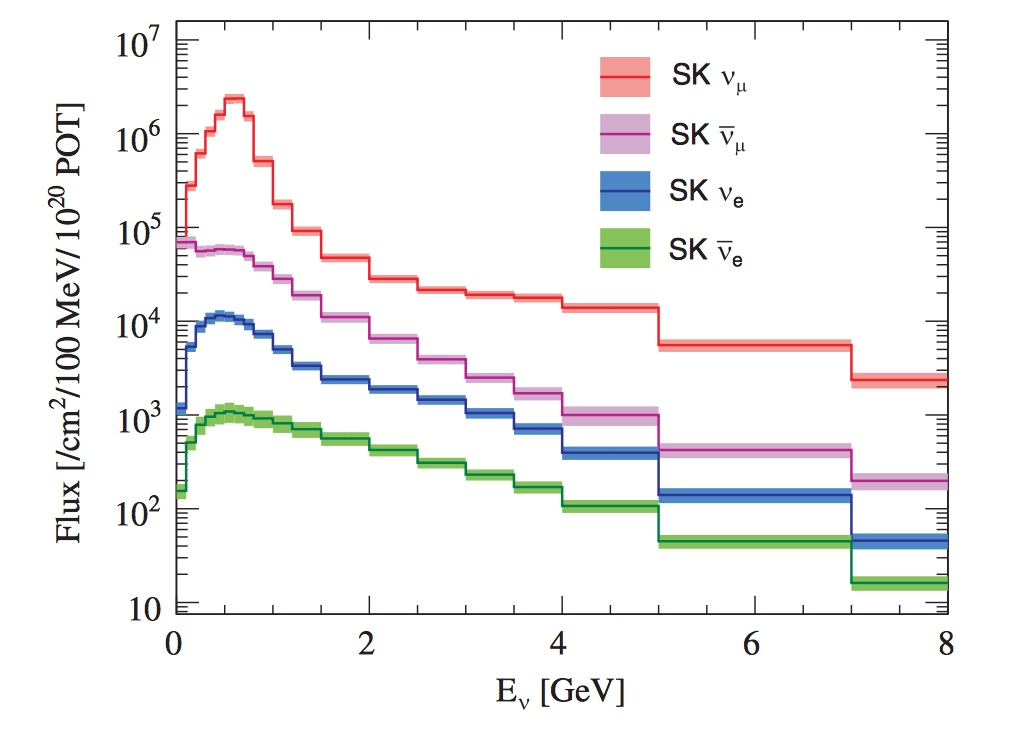
\includegraphics[width=\textwidth]{figures/ND280Flux.jpeg}
\vspace{2mm}
\caption{Simulated unoscillated expected neutrino fluxes for various flavours with expected systematic before applying near detector data plotted as bands. at Super-K~\cite{21T2K}.}
\label{fig:ND280Flux}
\end{figure}

\begin{figure}[h!]
\centering
  \centering
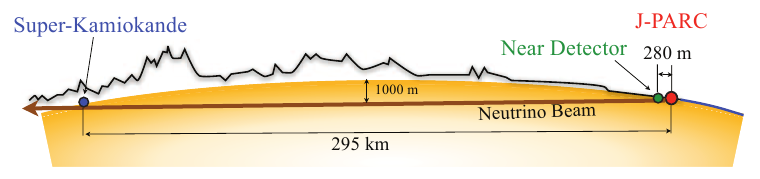
\includegraphics[width=\textwidth]{figures/T2KBeam.png}
\vspace{2mm}
\caption{A schematic view of the T2K experiment, including the near detector site ND280 and Super-K.}
\label{fig:T2K}
\end{figure}

The near detector hall contains two main experiments, an on-axis experiment INGRID and the off-axis ($2.5\deg$) ND280 detector both used to reduce model uncertainty and systematic uncertainty in the Super-Kamiokande analysis. \textbf{More details?}

The experiment wanted to improve the understanding of the neutrino oscillation parameters. T2K was able to successfully observe the appearance of muon to electron neutrino oscillations and find evidence that the third mixing angle $\theta_{13}$ is not zero. This is still an ongoing experiment. 

\begin{figure}[h!]
\centering
  \centering
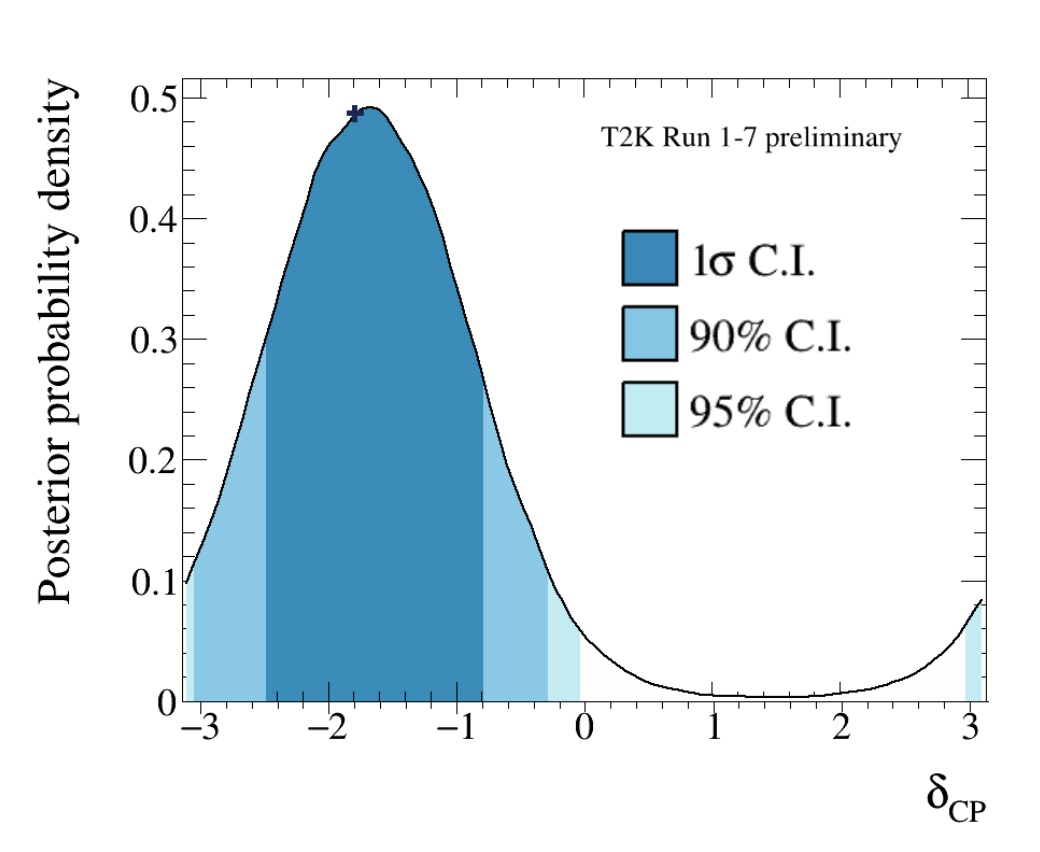
\includegraphics[width=0.7\textwidth]{figures/t2k1.jpeg}
\vspace{2mm}
\caption{Posterior probability density on $\delta$CP, where the cross represent the best-fit~\cite{T2Kfigures}.}
\label{fig:T2KCP}
\end{figure}

\begin{figure}[h!]
\centering
  \centering
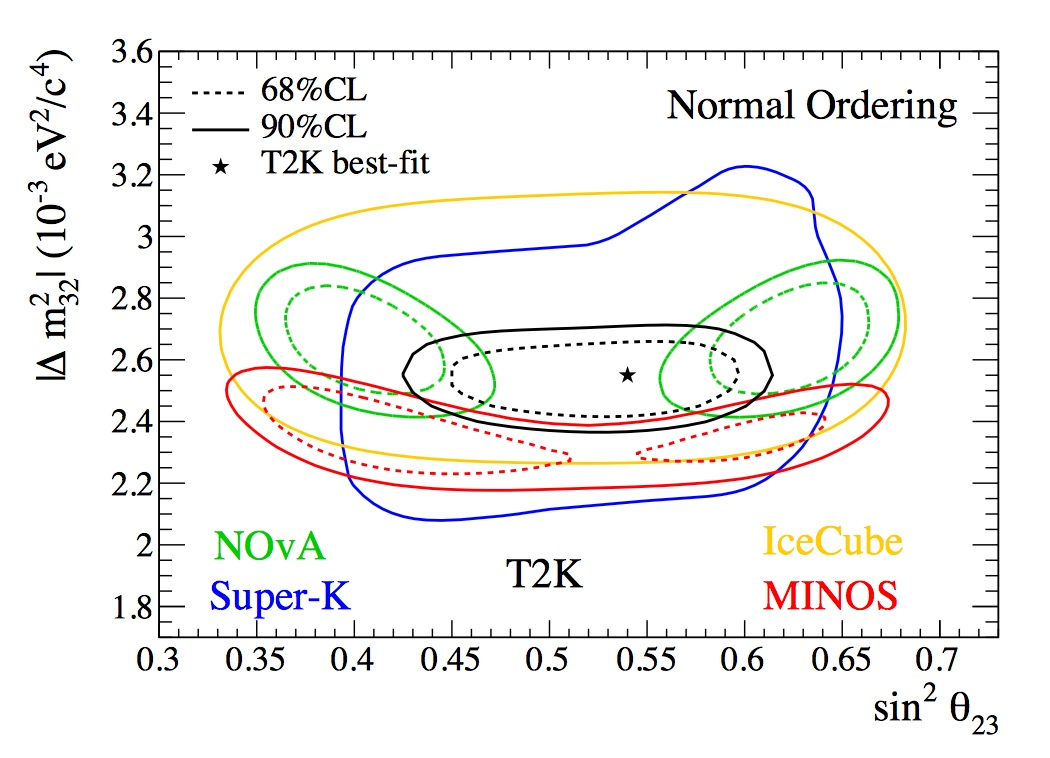
\includegraphics[width=0.7\textwidth]{figures/t2k2.jpeg}
\vspace{2mm}
\caption{The 90\% and 68\% confidence levels in the $\sin ^2 \theta_{23}-\Delta m^2_{32}$ space from T2K compared to other experiments, assuming normal ordering of neutrino masses~\cite{T2Kfigures}.}
\label{fig:T2K23}
\end{figure}

The main source of systematic error for T2K is caused by the difference of the target material and acceptance between the ND280 near detector (hydrocarbon) and the far detector water Cherenkov detector~\cite{T2Kpaper} motivating further studies and upgrades to the ND280 detector.

\section{Reactor}
Nuclear reactors are very intense sources of low energy neutrinos. Through beta-decay channels electron neutrinos are produced with well known energy spectra and low background. Compared to other neutrino sources the energy range is limited to below $9 MeV/c$, see \FigRef{fig:reactor} as well as a harsh cut of at $1.8 MeV/c$ required for inverse beta decay to occur. The low energy range means that oscillation experiments can be performed with a short baseline since equation~\ref{eq:twoPNeutrinoosc} provides the same probability by decreasing both the momentum and baseline.

The low energy range also means that experiments based on reactor neutrinos can only search for $\bar{\nu_e}$ disapperence since the produced neutrinos do not have enough energy to produce muons or taus and any neutral current interaction will be very difficult to distinguish form background. Based on the current values neutrino reactor experiments are well suited to determine $\theta_{12}$ and $\Delta m_{12}^2 $ as well as  $\theta_{13}$ and $\Delta m_{13}^2 $.

\begin{figure}[h!]
\centering
  \centering
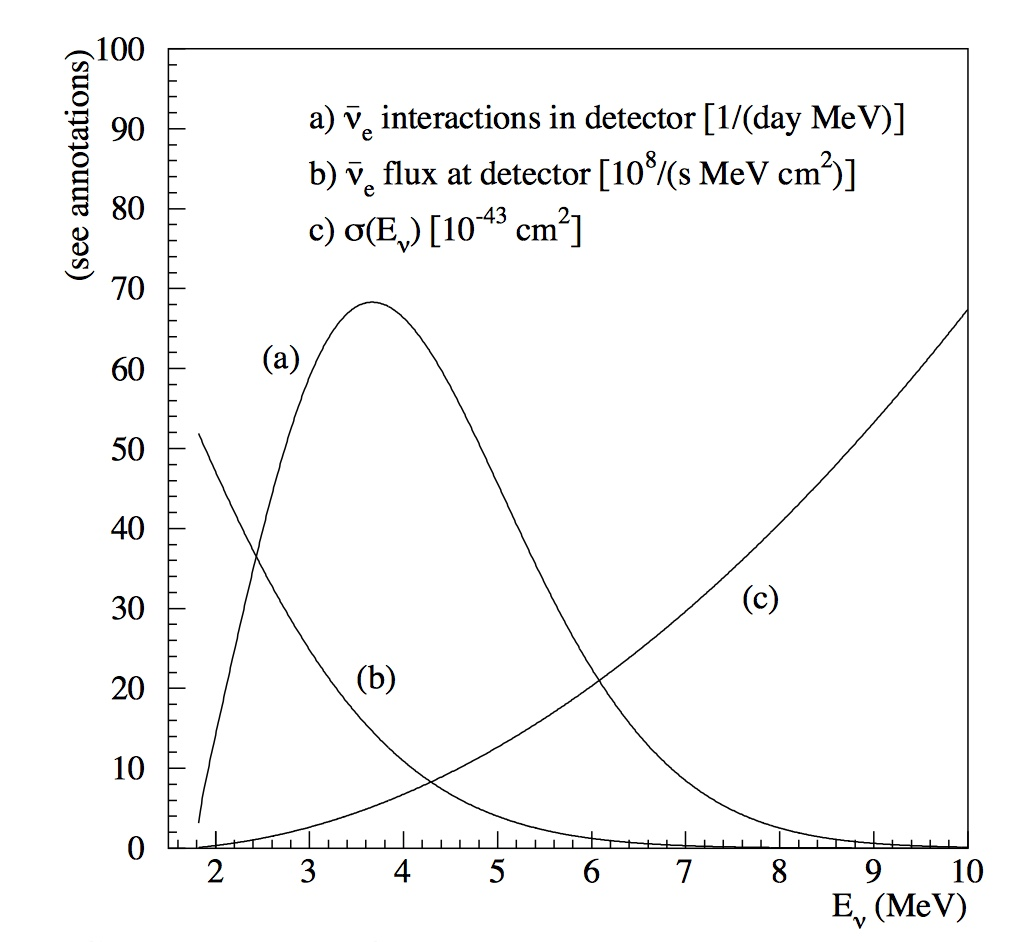
\includegraphics[width=0.7\textwidth]{figures/reactor.jpeg}
\vspace{2mm}
\caption{Energy spectrum of $\bar{\nu_e}$, the inverse beta decay cross section and interaction spectrum of detected inverse beta decay events~\cite{65Reactor}.}
\label{fig:reactor}
\end{figure}

\subsection{KamLAND}
Kamioka Liquid Scintillator Antineutrino Detector (KamLAND)

KamLAND, the Kamioka Liquide scintilator Anti-Neutrino Detector, was build in 2002 and helped investigate if there were any neutrino oscillations by looking at anti electron neutrinos emitted from distant reactors~\cite{46KamLAND}.

\subsection{Double Chooz}
\textbf{Correct after Pauls comments and add data.}

The Double Chooz experiment~\cite{45DoubleChooz} used anti-neutrinos produced two nuclear cores from a nuclear power station to improve the neutrino mixing angle $\theta_{13}$ as well as showed that these detectors can be used to ensure non-proliferation~\cite{66ReactorNP}. The experiment consisted of two Cherenkov detectors at a distance of 280m and 1050m both consisted of PMTs inside a scintillating volume shielded from cosmic radiation. 

\begin{figure}[h!]
\centering
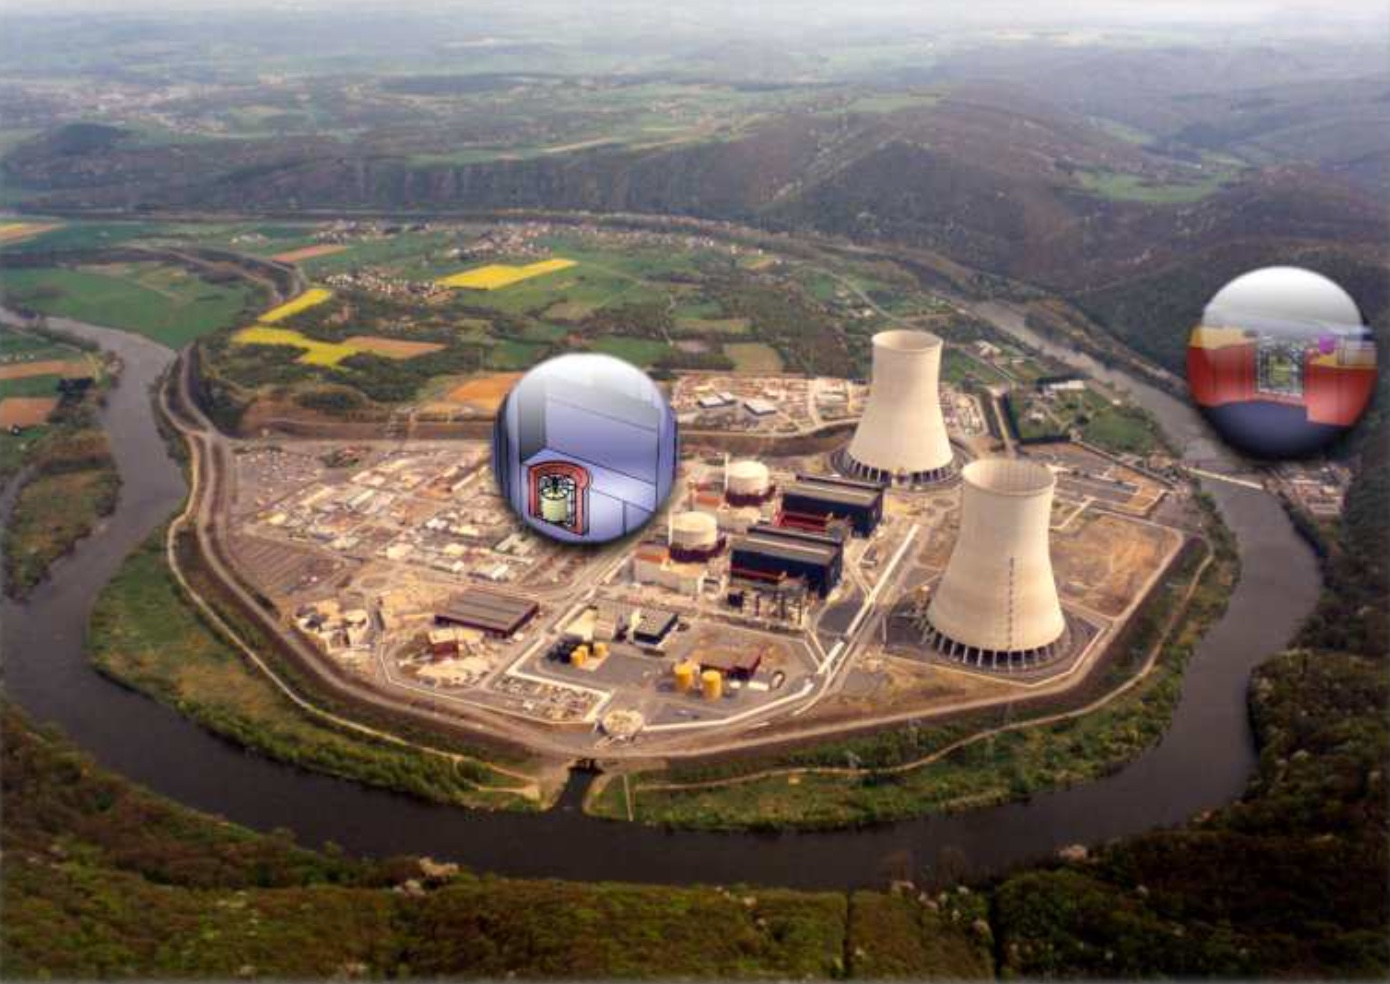
\includegraphics[width=0.6\textwidth]{figures/doubleChooz.jpeg}
\caption{Overview of the Double Chooz experimental site~\cite{45DoubleChooz}.}
\label{fig:dc}
\end{figure}

\subsection{Daya Bay}
\textbf{Correct after Pauls comments and add data.}

The Daya Bay experiments~\cite{44DayaBay}, main goal is to improve the measurement of $\theta_{13}$It is improving results from Double Chooz by utilizing eight identical detectors placed at three locations around the Daya Bay area consisting of a total of 6 different nuclear cores. Each detector is a Cherenkov detector using PMTs.

\begin{figure}[h!]
\centering
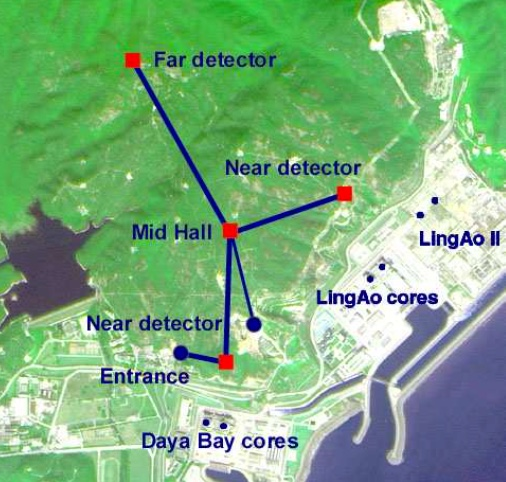
\includegraphics[width=0.4\textwidth]{figures/DayaBay.jpeg}
\caption{Layout of the Daya Bay experiment.~\cite{44DayaBay}.}
\label{fig:DB}
\end{figure}

\subsection{RENO}

\subsection{JUNO}

\section{Future neutrino oscillation experiments}
\textbf{Correct after Pauls comments and add data.}

\subsection{Hyper-K}
\textbf{Correct after Pauls comments and add data.}

The Hyper-Kamiokande Experiment\cite{24HyperK}  builds on the T2K-experiment\cite{21T2K} by improving the neutrino beam at JPARC, and expanding the water Cherenkov detector by a factor of 10 to a fiducial volume of 500 ktons, which aims to improve the sensitivity for $\delta_{cp}$.


\subsection{DUNE}
\textbf{Correct after Pauls comments and add data.}

LBNF/DUNE\cite{23DUNE} is a new experiment aiming at looking at the full range of $\delta_{cp}$ with greater sensitivity than before by improving on the MINOS~\cite{MINOS} experiment, and performing an electron neutrino appearance measurement with a high-powered neutrino beam from Fermilab and a 40 kton liquid argon detector at a distance of 1300 km, in the Homestake mine in South Dakota.

\section{Neutrino Factory}\label{subsec:nuFACT}
\textbf{Correct after Pauls comments and add data.}

The Neutrino Factory (NuFACT) is a novel concept for a neutrino accelerator which will produce a high intensity (1000 higher than previously) and high energy beam (up to 20-50 GeV). Compared to other previous experiments it will produce a two flavour, electron and muon, neutrino beam through a muon decay ring. The neutrino factory has the capacity to improve the precision of neutrino oscillation measurements, since the neutrino beam from the decay of muons can be determined with high accuracy. The beam produces one bunch of $\mu^+$ and one bunch of $\mu^-$, so the facility can make measurements of $\nu_{\mu}$ and $\bar{\nu_{e}}$ and $\bar{\nu_{\mu}}$ and $\nu_{e}$ simultaneously. Using this $\delta_{cp}$ can be decisively explored, with an expected accuracy of $\Delta \delta_{CP}\sim 5^\circ$~\cite{25NUfact}. NuFACT is also significantly better that alternative facilities at measuring the value if $\theta_{13}$ is small. A schematic of the facility is shown in figure \ref{fig:nuFact} showing the full accelerator chain. The full chain, starts by producing muons and pions from a proton beam on target. The particles are selected based on charge in a magnetic horn after which the pions decay into muons in a transport line before the beam being collating to form a pure muon beam. The muon beam is then cooled to focus the beam before further accelerating the muon beam to its final energy and introducing it into the decay ring. After $\approx 70$ turns of the circuit the muons decay through the following modes with the branching ratio:

\begin{align}
\mu^- &\rightarrow e^- + \bar{\nu_e} + \nu_\mu, \approx 100\% \\
\mu^- &\rightarrow e^- + \bar{\nu_e} + \nu_\mu + \gamma, <1\% \\
\mu^- &\rightarrow e^- + \bar{\nu_e} + \nu_\mu + e^+ + e^-, <1\%
\end{align}

From the branching ratio the energy spectrum and competition of the neutrino beam is well known, The beam is also produced as a pure beam since they are two neutrino flavours at the same time but with different flavours. It is important to know that a muon beam will only produce muon neutrinos and anti-electron neutrinos. Thus any electron neutrinos or anti-muon neutrinos discovered must have been produced through oscillation. Currently there are proposals for NuFACT to be constructed at CERN~\cite{25NUfact}, ESS~\cite{ESS} and FERMILAB~\cite{NuFACTfermi}, where it is also seen as a step toward a full muon collider experiment.
%Neutrino factory, explain it. MIND detector for nufact.  MIND needed for charge id, wrong sign muons produced from mu neutrino and anti electron neutrino in accelerator, anti electron to anto muon oscillation. Nufact known 0 anti nu mu in generation, only in oscillation. Prob is 0 for nufact for wrong sign at near detector/source.

\begin{figure}[h!]
\centering
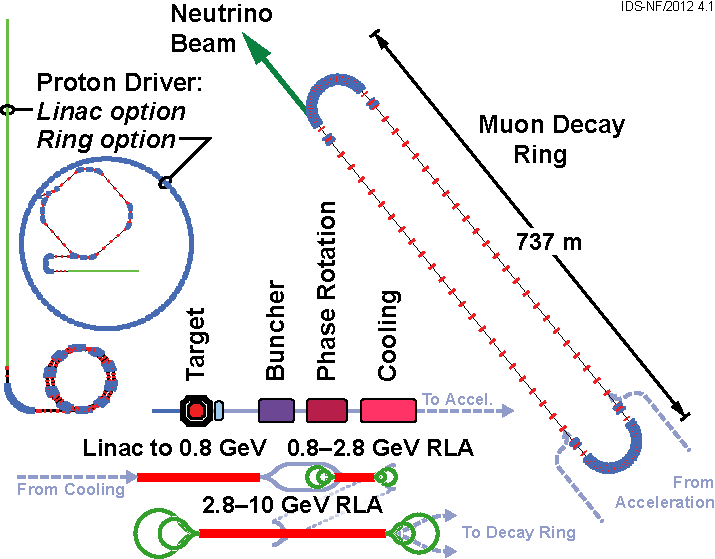
\includegraphics[width=0.9\textwidth]{figures/131112-IDS-NF.pdf}
\caption{Schematic diagram of the Neutrino Factory~\cite{Fix7}.}
\label{fig:nuFact}
\end{figure}

\begin{figure}[h!]
\centering
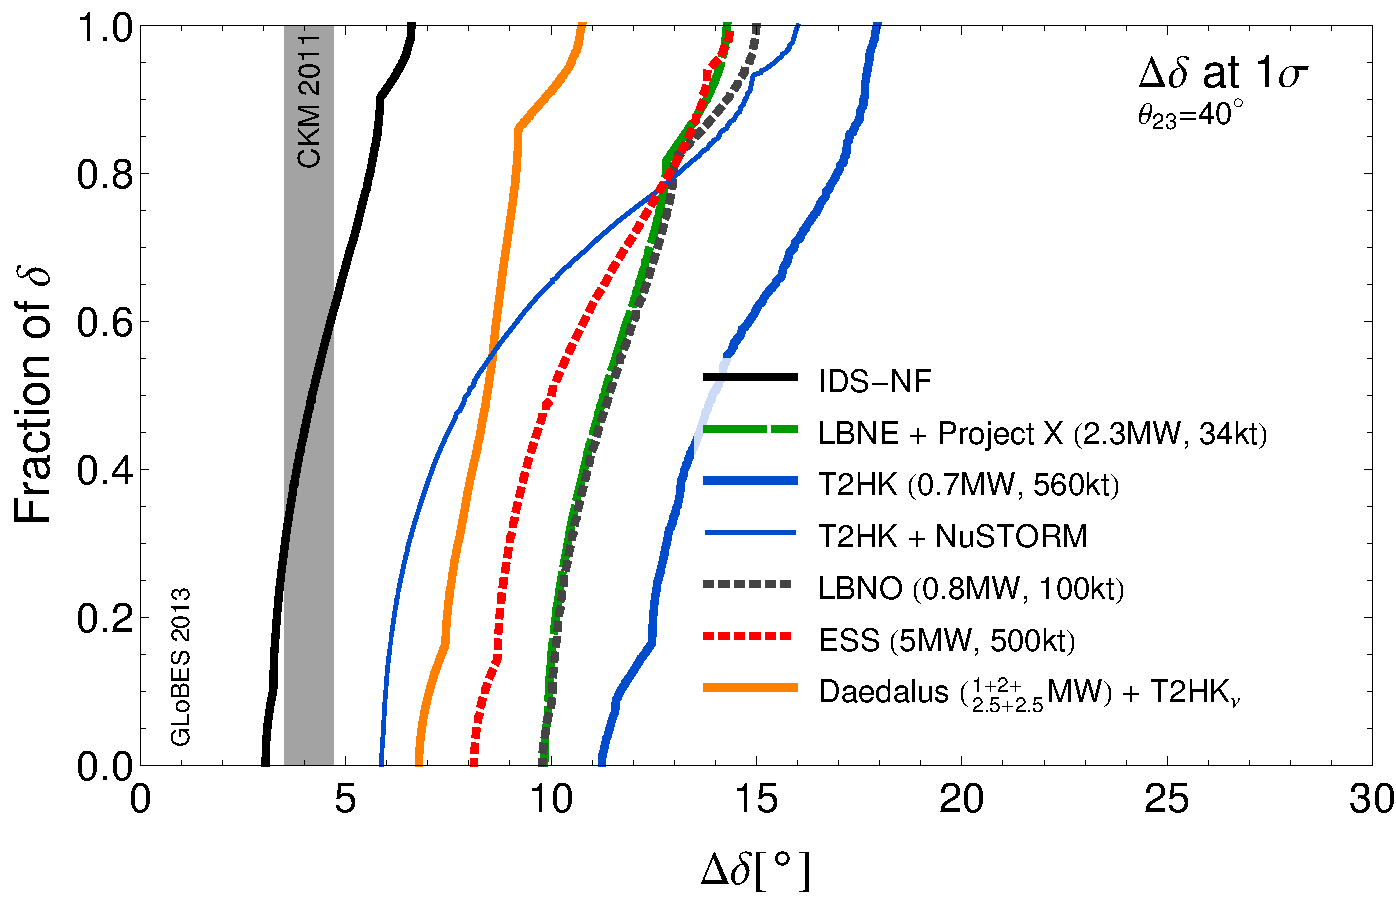
\includegraphics[width=0.9\textwidth]{figures/rdr-cp-precision-comparison-131216.pdf}
\caption{Expected precision for a measurement of the $\delta_{cp}$ at a Neutrino Factory compared to alternate neutrino oscillation facilities~\cite{Fix7}.}
\label{fig:nuFactExp}
\end{figure}

The Neutrino Factory is an complex and expensive facility which requires new technology to be realised. To overcome this a staged approach has been suggested, where each stage would be delivering physics~\cite{Fix7}. The first state in this plan is named nuSTORM (Neutrinos from Stored Muons) with a schematic shown in figure~\ref{fig:nuStorm}. The nuSTORM beam is designed to produce 3.8 GeV/c muons which are injected into a muon storage ring. Compared to the full neutrino factory nuSTORM is expected to have some pions and kaons in the final beam producing both neutrinos and anti-neutrinos for both muon and anti-muon modes and thus a near detector is required to measure the flux of both. 

\begin{figure}[h!]
\centering
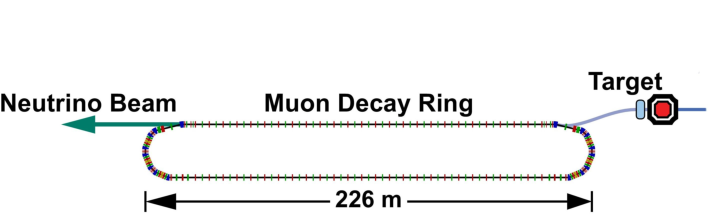
\includegraphics[width=\textwidth]{figures/nuSTORM_schematic.pdf}
\caption{A schematic of a nuSTORM facility~\cite{Fix7}.}
\label{fig:nuStorm}
\end{figure}

For the both NuFACT and nuSTORM the detector type proposed will be a MIND type, similar to the ones used in CDHSW and MINOS~\cite{NuFACTIDS}.

\textbf{Add in different channels and how it requires a charge identification to be able to identify the various challenge.}



\subsection{NuStorm}

\section{Magnetized Iron Neutrino Detectors}\label{subsec:MINDdetector}
\textbf{Correct after Pauls comments and add data.}

Magnetized Iron Neutrino Detectors (MINDs) have been operated in several experiments such as CDHSW~\cite{40CDHSW} and MINOS~\cite{MINOS}. This type of detector, with magnetized steel plates and scintillation plates, is well suited to provide large mass for neutrino experiments and is able to provide momentum measurements by using range and curvature calculations as well as providing charge identification. A MIND type detector has been selected as the baseline detector for a neutrino factory~\cite{ISS, 27Bross}, since it is the cheapest and most effective way of producing a large magnetized volume. This has provided the motivation for creating a prototype detector to perform a number of studies.

Since water Cherenkov and liquid argon detectors have been established or actively studied for future very large scale neutrino oscillation experiments, a MIND type detector is not foreseen to be used as the main interaction medium for any planned upcoming experiments.. A MIND type detector can however be used to provide charge identification of muons if positioned downstream of any neutrino target which is not magnetized.


\textbf{OLD}

\subsubsection{IceCube}
The IceCube observatory~\cite{43IceCube} also exploits the fact that particles produced in neutrino interactions emit Cherenkov photons. The low interaction probability of neutrinos require a large interaction volume. The South Pole offers a large interaction volume with very good optical qualities, using this is possible to instrument cubic kilometres of ice with a rather sparse spacing of detectors. The basic detection unit in IceCube is the digital optical module (DOM). The DOM contains, amount other things a PMT encapsulated in a glass pressure sphere to withstand the extreme pressure in the deep ice. In total 5160 DOMS are deployed, instrumenting a volume of one cubic kilometre of ice and allowing detection of astrophysical neutrinos in the energy range of TeV to PeV.

\begin{figure}
\centering
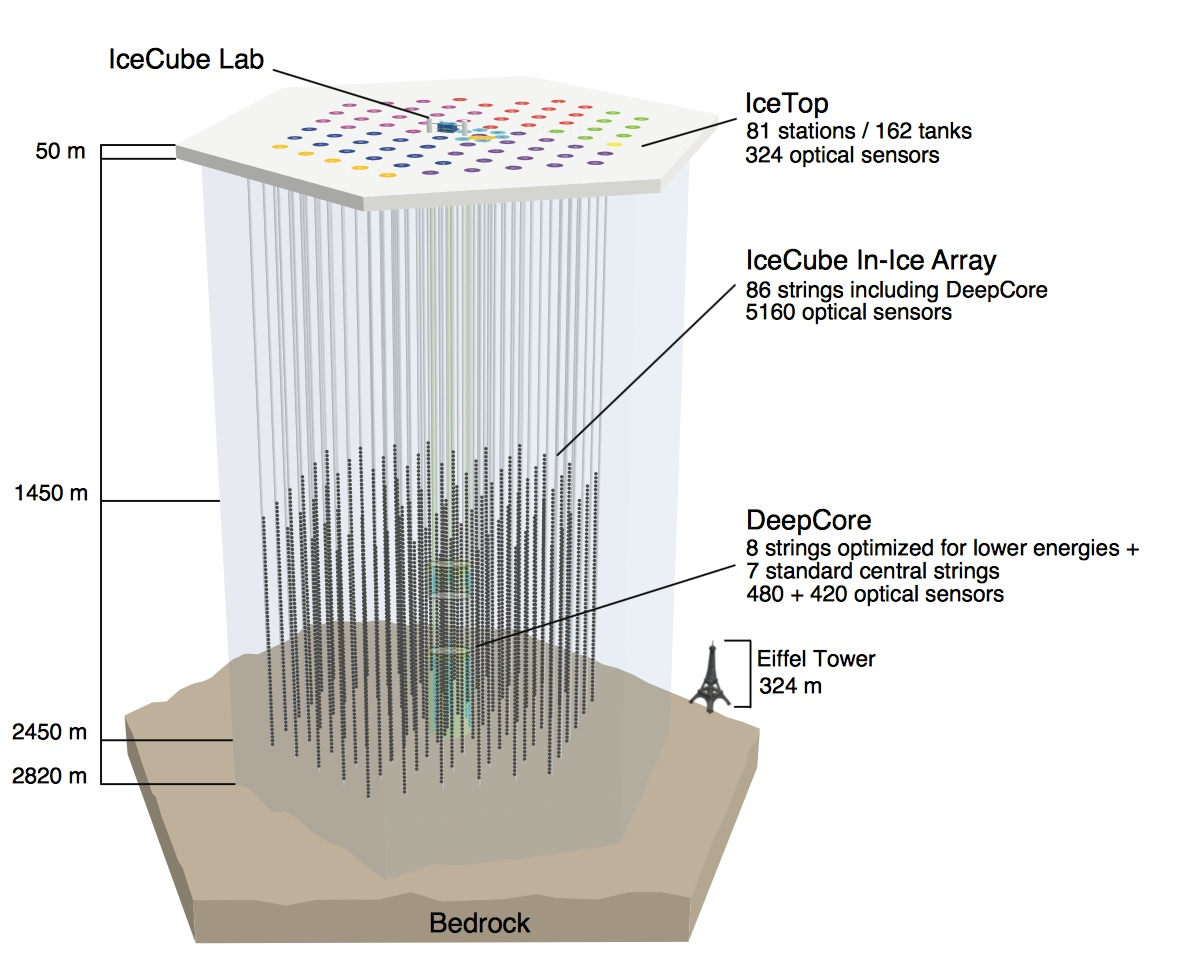
\includegraphics[width=.5\textwidth]{figures/IceCube.jpeg}
\caption{The IceCube Neutrino Observatory}
\end{figure}







%==============================================================================
